% Based on template by MR

\documentclass[12pt,twoside,notitlepage]{report}

\usepackage{a4}
\usepackage{verbatim}
\usepackage{natbib}
\usepackage{graphicx}
\usepackage{algorithm}
\usepackage{bm}

\input{epsf}                            % to allow postscript inclusions

\raggedbottom                           % try to avoid widows and orphans
\sloppy
\clubpenalty1000%
\widowpenalty1000%

\addtolength{\oddsidemargin}{6mm}       % adjust margins
\addtolength{\evensidemargin}{-8mm}

\renewcommand{\baselinestretch}{1.1}    % adjust line spacing to make
                                        % more readable

% Resize over-large graphics ( http://tex.stackexchange.com/questions/27083/can-i-conditionally-scale-an-image-with-graphicx )
\newcommand{\lwincludegraphics}[2][]{%
  \sbox{0}{\includegraphics[#1]{#2}}%
  \ifdim\wd0>\linewidth
    \resizebox{\linewidth}{!}{\box0 }%
  \else
    \leavevmode\box0
  \fi}

\newcommand{\msg}[1] {{\bf #1}}         % \msg command for formatting Paxos messages
\newcommand{\op}[1]  {{\bf #1}}         % \op  command for formatting database operations
\newcommand{\superscript}[1]{\ensuremath{^{\textrm{#1}}}}
\newcommand{\subscript}[1]{\ensuremath{_{\textrm{#1}}}}


\begin{document}

\bibliographystyle{plain}


%%%%%%%%%%%%%%%%%%%%%%%%%%%%%%%%%%%%%%%%%%%%%%%%%%%%%%%%%%%%%%%%%%%%%%%%
% Title


\pagestyle{empty}

\hfill{\LARGE \bf Charlie Shepherd}

\vspace*{60mm}
\begin{center}
\Huge
{\bf PDB: A Distributed Database Based on Paxos} \\
\vspace*{5mm}
Computer Science Tripos \\
\vspace*{5mm}
Churchill College \\
\vspace*{5mm}
\today  % today's date
\end{center}

\cleardoublepage

%%%%%%%%%%%%%%%%%%%%%%%%%%%%%%%%%%%%%%%%%%%%%%%%%%%%%%%%%%%%%%%%%%%%%%%%%%%%%%
% Proforma, table of contents and list of figures

\setcounter{page}{1}
\pagenumbering{roman}
\pagestyle{plain}

\chapter*{Proforma}

{\large
\begin{tabular}{ll}
Name:               & \bf Charlie Shepherd                        \\
College:            & \bf Churchill College                     \\
Project Title:      & \bf PDB: A Distributed Database Based on Paxos \\
Examination:        & \bf Computer Science Tripos, July 2013        \\
Word Count:         & \bf wordcount \\
Project Originator: & Charlie Shepherd                    \\
Supervisor:         & Stephen Cross                    \\
\end{tabular}
}


\section*{Original Aims of the Project}

\subsection*{Project aims}

I aim to implement a distributed database. This will be based on the Paxos protocol.

\subsubsection*{Paxos}

The first half of the project is to implement the Paxos protocol. This will be done in a module,
providing an interface which the database can then use to

The project must correctly implement the Paxos protocol.  The library must be capable of forming a
running network, in particular dynamic leader election, as well as achieving consensus on a
key/value store across the network.

The database must implement a subset of SQL, specifically. The database must have all ACID
properties, that is.

\section*{Work Completed}

All that has been completed appears in this dissertation.

\section*{Special Difficulties}

None.

\newpage
\section*{Declaration}

I, Charlie Shepherd of Churchill College, being a candidate for Part II of the Computer Science
Tripos, hereby declare that this dissertation and the work described in it are my own work,
unaided except as may be specified below, and that the dissertation does not contain material that
has already been used to any substantial extent for a comparable purpose.

\bigskip
\leftline{Signed: }

\medskip
\leftline{Date: \today}

\cleardoublepage

\tableofcontents

\listoffigures

\newpage
\section*{Acknowledgements}

Acknowledge various people

%%%%%%%%%%%%%%%%%%%%%%%%%%%%%%%%%%%%%%%%%%%%%%%%%%%%%%%%%%%%%%%%%%%%%%%
% now for the chapters

\cleardoublepage        % just to make sure before the page numbering
                        % is changed

\setcounter{page}{1}
\pagenumbering{arabic}
\pagestyle{headings}

\chapter{Introduction}

\section{Overview}

``The Paxos algorithm, when presented in plain English, is very simple.'' \cite{lamport01}. \\
Despite this assertion, Paxos has a reputation for being hard to implement. Both
\emph{Paxos Made Live} \cite{chandra07} and \emph{Paxos Made Moderately Complex} \cite{renesse11}
repeatedly show how intricate implementing a Paxos actually is.

With this in mind I set out to build a distributed database based on the Paxos protocol.

% Paxos is a consensus algorithm for distributed systems. It was first described in Leslie Lamport's
% paper \emph{The Part Time Parliament} \cite{lamport98}. It has been used by Google and Yahoo in
% their internal services as the basis of large scale distributed systems.

\section{Motivation}

Paxos is a complex protocol, and one that is notoriously subtle. I took on the challenge of not
only implementing it, but also designing and coding a database layer on top. I wanted this
database to be functional, and have the properties expected of a standard database solution. This
includes SQL, transactions and ACID properties.

\section{Distributed Consensus Problem}

Consensus is an integral problem in distributed systems. The consensus problem is that of getting
all nodes in a distributed system to agree on a value. Formally, an algorithm that satisfies the
consensus problem satisfies three properties:

\begin{enumerate}
\item Agreement - all nodes must decide the same value.
\item Validity - the value that is decided upon must have been proposed by some node in the
	network.
\item Termination - all nodes eventually decide on a value.
\end{enumerate}

Decision is defined as follows - a process must decide on a value only once, and cannot change the
value once it has been decided.

\subsection*{Failure Modes}

Distributed networks must be able to deal with failure in a number of forms. Nodes may fail and
stop executing completely, this is known as the \emph{fail-stop} model. In practice, a more accurate
model is the \emph{fail-recover} model. This is where a node stops executing, then resumes execution
at a later time. This more accurately models real life, where asynchronous networks mean that it
may take an arbitrarily long time to receive a message, and that messages may arrive out of order
or not at all. The most general failure model is that of \emph{Byzantine failure}, where nodes may
respond incorrectly or even deliberately lie in order to mislead the protocol. In practice this is
unlikely, and can be mediated using checksums, message digests and authentication. In the
Preparation chapter I will go into detail about the types of failure that my database can handle.

\subsection*{2 Phase Commit}

% S comment: too detailed, move to preparation and discuss what 2pc tries to achieve and its flaws
% rather than details

2 Phase Commit is one of the simplest protocols that aims to solve the Distributed con

\subsection*{3 Phase Commit}


\subsection*{Paxos}

% http://betathoughts.blogspot.co.uk/2007/06/brief-history-of-consensus-2pc-and.html
% The kernel of Paxos is that given a fixed number of processes, any majority of
% them must have at least one process in common. For example given three
% processes A, B and C the possible majorities are: AB, AC, or BC. If a decision
% is made when one majority is present eg AB, then at any time in the future when
% another majority is available at least one of the processes can remember what
% the previous majority decided. If the majority is AB then both processes will
% remember, if AC is present then A will remember and if BC is present then B
% will remember.
%
% Paxos can tolerate lost messages, delayed messages, repeated messages, and
% messages delivered out of order. It will reach consensus if there is a single
% leader for long enough that the leader can talk to a majority of processes
% twice. Any process, including leaders, can fail and restart; in fact all
% processes can fail at the same time, the algorithm is still safe. There can be
% more than one leader at a time.
%
% Paxos is an asynchronous algorithm; there are no explicit timeouts. However, it
% only reaches consensus when the system is behaving in a synchronous way, ie
% messages are delivered in a bounded period of time; otherwise it is safe. There
% is a pathological case where Paxos will not reach consensus, in accordance to
% FLP, but this scenario is relatively easy to avoid in practice.

Paxos is a generalisation of 2PC and 3PC that handles more failure modes. While 3PC can handle
failures, it only handles \emph{fail-stop} failures, not \emph{fail-recover} failures. This is
unfortunate, as computer networks are asynchronous networks, and can therefore be modelled using a
fail-recover model to account for arbitrary delays from messages being sent to being received
(fail-stop would mean messages can only be dropped, not delayed for an arbitrary length of time).

Paxos relies on the fact that any majority $M$ has at least one member in common. Therefore if we
enforce the constraint that any decision must be made by a majority, then once a decision is made,
in any subsequent decision there will be at least one member who was present in the previous
decision. This is the central tenet of Paxos, where a majority is known as a \emph{quorum}.

A key advantage of Paxos is that it can guarantee consistency during network partitions,
unlike 3PC which gives availability instead.

However, a potential drawback is that Paxos has a pathological case where it will not make
progress, ie, there is no upper bound on the time it will take to achieve consensus (it may never
terminate). This is due to the FLP impossibility proof \cite{fischer85}, which states that it is
impossible to guarantee liveness in an asynchronous network where there is at least one failure.
In practice it is a situation that is relatively easy to avoid, and is not a serious concern.

\section{Databases}

\subsection*{ACID}

Commonly all databases provide ACID properties. ACID stands for:

\begin{itemize}
\item Atomic - an operation is either performed in its entirety or is not performed at all.
\item Consistent - the database remains in a \emph{consistent} state at all times, where being
	consistent is defined as being valid according to rules that ensure database integrity.
\item Isolated - one operation cannot see the intermediate state due to another operation occurring
	at the same time.
\item Durable - once an operation is ``committed'' it is permanently stored - the effects of it will
	not be lost.
\end{itemize}

There are many reasons why ACID is a key requirement of most databases. ACID makes it far easier
for application developers to reason about concurrency in a system where there may be multiple
clients reading and writing the same data simultaneously. It also enable effective abstraction, as
the atomicity requirement in particular gives the well defined characteristics when an operation
or transaction fails. ACID also provides clear guarantees with regard to data stability and
longevity, in particular how this relates to consistency, so that users can be clear as to the
overall state of the system.

\subsection*{Centralisation vs Distributed}

Databases are generally found in one of two topologies - centralised or distributed. These
different topologies are used in different situations and to different ends.

A centralised database is a single node in a single location.
% S comment: reasons? citation? (for sentence below)
In general, centralised databases are simpler in design and on the whole faster than distributed
databases.
Many general properties of centralised vs. distributed systems apply to centralised databases -
they are easier to perform organise, to edit, to query and to backup. May slow down under load. It
is easier to maintain the integrity of data on a centralised database, as there is only one
``current'' version of the data under consideration.

In contrast, distributed databases are more resilient and scalable than centralised databases.
There is no longer a single point of failure, and they can be extended by adding nodes, although
this will have a point of diminishing returns. Distributed databases are often more complex in
design, as they have to ensure consistency between nodes \footnote{although there is a recent trend to
relax this constraint in certain ``NoSQL'' databases. Here I will only consider traditional RDBMS
systems.} In particular, distributed databases can be slow accessing non local data.

% S comment: in particular distributed is a generalisation of centralised

\subsection*{Existing Paxos databases}

Paxos has recently become a very popular algorithm for ensuring distributed
consensus. One good example is Google using Paxos for a distributed lock
service called ``Chubby'' \cite{chandra07}. This underpins their BigTable
distributed database which is used across Google.

Apache Zookeeper, a centralised service for providing distributed services such
as synchronisation, naming and configuration management, also uses a Paxos
based protocol called ZAB.

% S comment: try to expand this section, giving more details about the implementation

\cleardoublepage

\chapter{Preparation}

\section{Requirements Analysis}

Given the brief to design and create a protocol and a database there is a huge amount of scope for
variety in the project. Requirements Analysis narrows down the purpose of a project to formal
goals which can easily be objectively verified against the finished project.

\subsection*{Paxos}
\paragraph{Correctness} Above all, the implementation of Paxos must be correct. This means that it
must conform to the description of the algorithm specified in \emph{The Part Time Parliament}.
\paragraph{Dynamic node membership} The implementation of Paxos must be able to support nodes
joining and leaving dynamically without losing correctness.

\subsection*{Database}
\paragraph{Encapsulation} The database must be a separate module to Paxos, and must be layered on
top of the API provided by the Paxos module.
\paragraph{Distributed} The database must be distributed. Any node in the network must have the
same capabilities as any other node in the network.
% homogenous
\paragraph{Transactions} The database must support transactions, which can be aborted, returning
the database to the state before the transaction was started. Transactions must operate in
isolation with each other.
\paragraph{ACID} The database must provide ACID properties. These are Atomicity, Consistency,
Isolation and Durability.
\paragraph{SQL} The interface to the database must be SQL. It may be a limited form of SQL, as the
main priority of the project is the protocol and database design, rather than the interface.

\section{Software Engineering}

In order for the project to be a success, clear software engineering practices must be followed.

\subsection{Development Technique}

There are a number of techniques for developing software. The classic software development
strategy is the Waterfall model. This follows the steps of Requirements and Specification, Design,
Implementation, Verification and Maintenance. I decided against using this and instead using the
Spiral Model. The Spiral Model uses the steps of the Waterfall model but repeats them several
times, iteratively working towards the final result.

The Spiral Model is more suitable for my project because although I have set out my formal
requirements, there is still a lot of uncertainty in the project. I have not designed a network
protocol or a database before and I have not implemented Paxos before. This means that it is
likely I will encounter unexpected difficulties in developing my project that may lead me to
change or shift my requirements. The Spiral Model is more flexible than the Waterfall Model in
this case.

\subsection{Language Choice}

There are many languages this project could be implemented in, but the two main choices were the
two languages I have the most experience in: C and Python. They are reasonably different languages
-- C is a compiled low-level language, while Python is an interpreted high level language. I
decided to use Python for a variety of reasons.

Python handles memory allocation internally, whereas whilst C provides great precision over memory
allocations, it also allows much more potential for memory handling errors. Python is more concise
than C and as a higher level language should allow me to develop several prototypes without being
impeded by focusing on details early on.

Also as my project is a network application, it should be mainly IO bound rather than CPU bound.
This means that the speed of the implementation language should not be a concern, as the speed
limitations of the implementation are unlikely to affect the performance of the project compared
to the limitations of the network.

\subsection{Module Dependencies}

Twisted is a Python framework used for event driven network programming. It contains support for
many different protocols, making writing efficient networking code a lot easier.  It is single
threaded, which means I will not have to worry about concurrency issues in my project. Twisted is
licensed under the MIT license so there are no license issues in using it for my project.

The other module I decided to use is PyParsing, a Python module for programmatically creating a
parser in Python. I decided to use this for parsing input SQL, as it will make the task
substantially simpler. I have already used PyParsing briefly, so I have a small amount of
familiarity with it. PyParsing is also distributed under the MIT license.

\subsection{Version Control and Backup}

Version control is a necessity in any software project. I decided to use a decentralised version
control system (DVCS) for a number of reasons. DVCSs have a distributed structure rather than
using a central or master server. This makes it possible to commit changes locally to a checkout
without needing a connection to any server. DVCSs also have advanced branching and merging tools,
making it easier to branch to develop experimental features, and then merge the feature in later.

Another advantage is being able to ``push'' the repository to any number of remote locations, as
an online copy or backup. In fact I used this as my backup strategy, keeping everything related to
my project in my repository and pushing every few hours to two different servers. This became very
helpful when my laptop broke and was unusable for a week. While it was being repaired I was still
able to work on my project without any difficulties. I simply cloned the repository from the
server copy onto the PWF computers and continued working.

While most DVCSs are very similar, I chose Git as it is the version control system I have the most
familiarity with.

\subsection{Testing}

In order to ensure I can have confidence that my project works correctly I will need to write
tests. I will write unit tests for the main modules of my project that will test its
functionality, both for expected input and also that it handles bad and malformed input correctly
and as expected. Tests are also useful for expressing the API usage of the different modules of
the project and checking that the interfaces connect sensibly. I will make sure I implement
regression testing, that is, every time there I fix a bug I will add a test ensuring any
regression causing the bug again will make the test fail.

I will run tests every time I make a commit, as they are quick to run and are a good confirmation
that the project is working as expected. Twisted has a unit testing framework that I will use as
it easily facilitates testing asynchronous programs, something that would be harder in other unit
testing frameworks available in Python.

\section{ACID}

ACID is an acronym for a set of properties that nearly all databases provide. These properties
provide certain guarantees about how the database handles transactions so that programmers using
the database can be confident that their transactions will be processed reliably. Here I will go
into some detail about what each of these properties mean.

\subsection*{Atomic}

Atomicity means that either an operation completes or it does not, there is no ``halfway'' state.
This means that the programmer using the database does not need to worry about cleaning up after
an operation, because if it does not succeed we can simply retry it without needing to worry about
the state it has left the database in. Atomicity also applies to transactions in the same way --
if we have a transaction as an operation composed of smaller single operations (for example, INCR
B, READ A $\rightarrow$ X, WRITE X + 10 $\rightarrow$ A), we don't want some of the operations to
complete and some not to. In this example, we may have the invariant $A = 10\times B$. If B was
incremented but then the transaction failed before A was updated, we would leave the database in
an invalid state.

\subsection*{Consistent}

Consistency is very closely related to atomicity, as consistency refers to a property of the
database, and atomicity refers to a property of operations performed on the database. In the
example used for atomicity, we had a constraint on the database (that $A = 10\times B$). We want
operations (or transactions) to transform the database from one consistent state to another. This
becomes more pertinent in distributed databases, as we may receive operations in one order at one
node, and in a different order at another node. If we apply the operations in the order that we
receive them, the two nodes are likely to be in inconsistent states.
% XXX do i wanna change this?

\subsection*{Isolated}

Isolation is the property that ensures that if one transaction is in the process of completing,
another transaction cannot see the intermediate state. Transactions should be processed as if they
were executed sequentially. It ensures that transactions that execute concurrently to each other
are also invisible to each other. This means a transaction should not be able to tell whether
another transaction is executing or not.

\subsection*{Durable}

The durable property refers to the permanence of a transaction. Once a database reports that a
transaction has been committed, it should persist in the database even in the face of power loss or
crashes. This is typically achieved by using a write-ahead log that is append only, so that in the
event of a crash, the database can reconstruct the state of all transactions reported as
``committed''. Distributed systems have an added complication of co-ordinating this property
across the network before the transaction can be reported as ``committed''.

\section{Distributed Consensus Protocols}

\subsection*{2 Phase Commit}

\begin{figure}[htb]
\centering
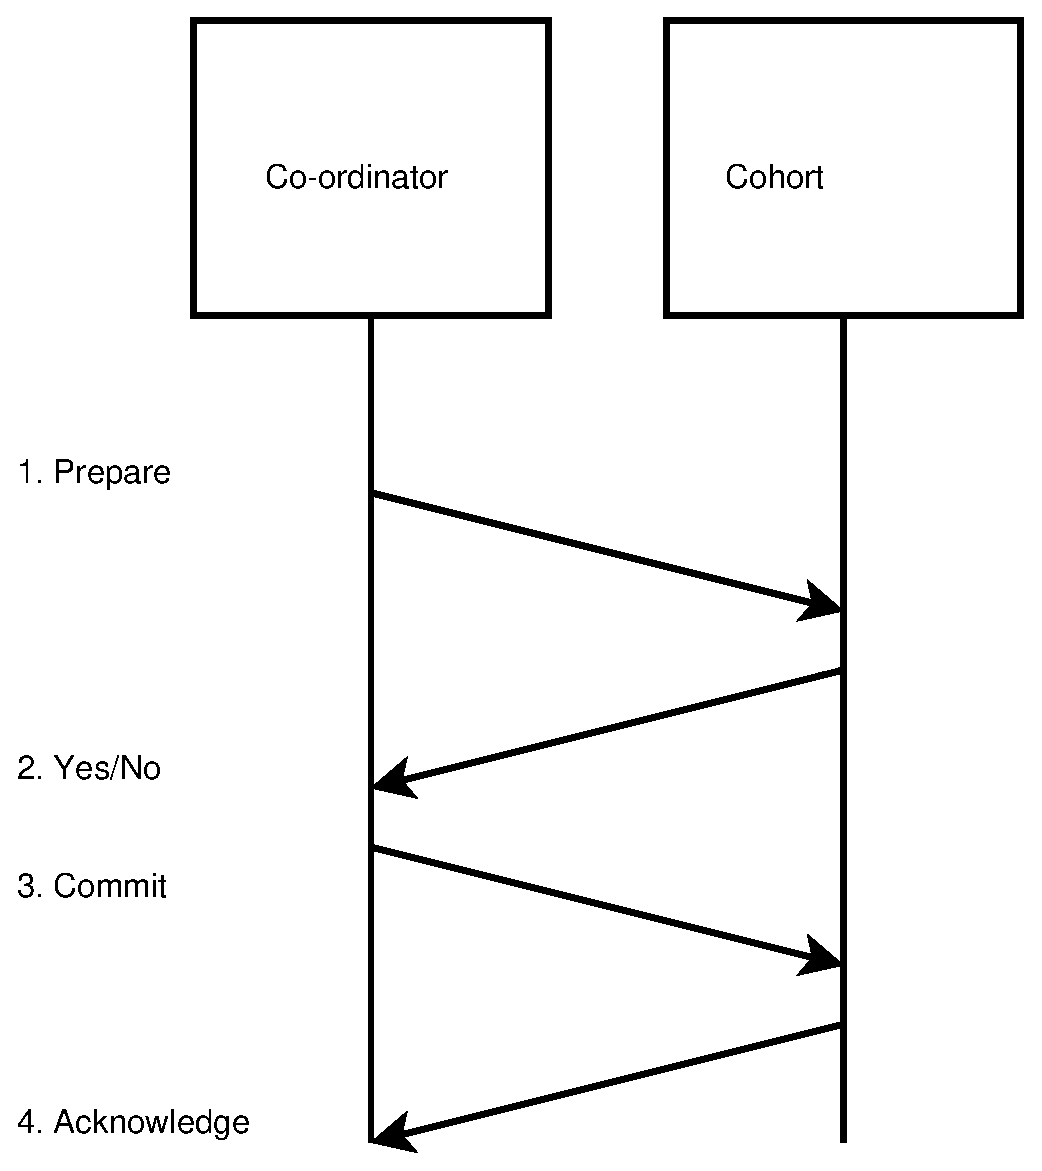
\includegraphics[scale=0.5]{figs/two-pc.eps}
\caption{\label{fig:two-pc}Two Phase Commit}
\end{figure}

2 Phase Commit (2PC) is one of the simplest consensus protocol, and one of the most brittle. The
basic message flow is shown in figure~\ref{fig:two-pc}. It has two phases:

\begin{enumerate}
\item The co-ordinator (the node initiating the protocol) sends a \msg{PROPOSE} message to each
	node in a cohort of size $N$, asking them to accept the value proposed.
\item The nodes reply with a \msg{YES} or \msg{NO} reply.
\item If all nodes respond with a \msg{YES} message, the co-ordinator sends a \msg{CONFIRM} message. Otherwise, if
	any node responds with a \msg{NO} message, it sends an \msg{ABORT} message to all nodes.
\item Nodes reply with an \msg{ACK} message, and the co-ordinator marks the transaction as
	complete when all nodes have acknowledged it.
\end{enumerate}

% S comment: split into 2 paragraphs and use footnotes

2PC solves the consensus problem in a failure free network. However if we can have failures then
the protocol can suffer from a number of limitations. If the co-ordinator crashes before sending
any messages, we satisfy consensus trivially. However, if the co-ordinator crashes after sending
$x$ messages, where $1 \le x < N$, the protocol cannot continue - it is blocked on the
co-ordinator resuming, and if it never resumes then some members of the cohort are blocked
permanently. In fact, once a node has sent a \msg{YES} message, it is blocked until it receives a
response. This is a big disadvantage for a concurrent system. While there are extensions to
resolve the problem of a crashing co-ordinator, these do not fix the fundamental problem of using
a blocking protocol in an asynchronous network. \footnote{These extensions often involve a ``watchdog'' or
``recovery'' node. This is still not a satisfactory solution as the simultaneous crash of the
co-ordinator and a cohort member means the state of the network is not recoverable (i.e., we cannot
tell if the cohort member who crashed voted \msg{YES} or \msg{NO}.)}

\subsection*{3 Phase Commit}

\begin{figure}[h!]
\centering
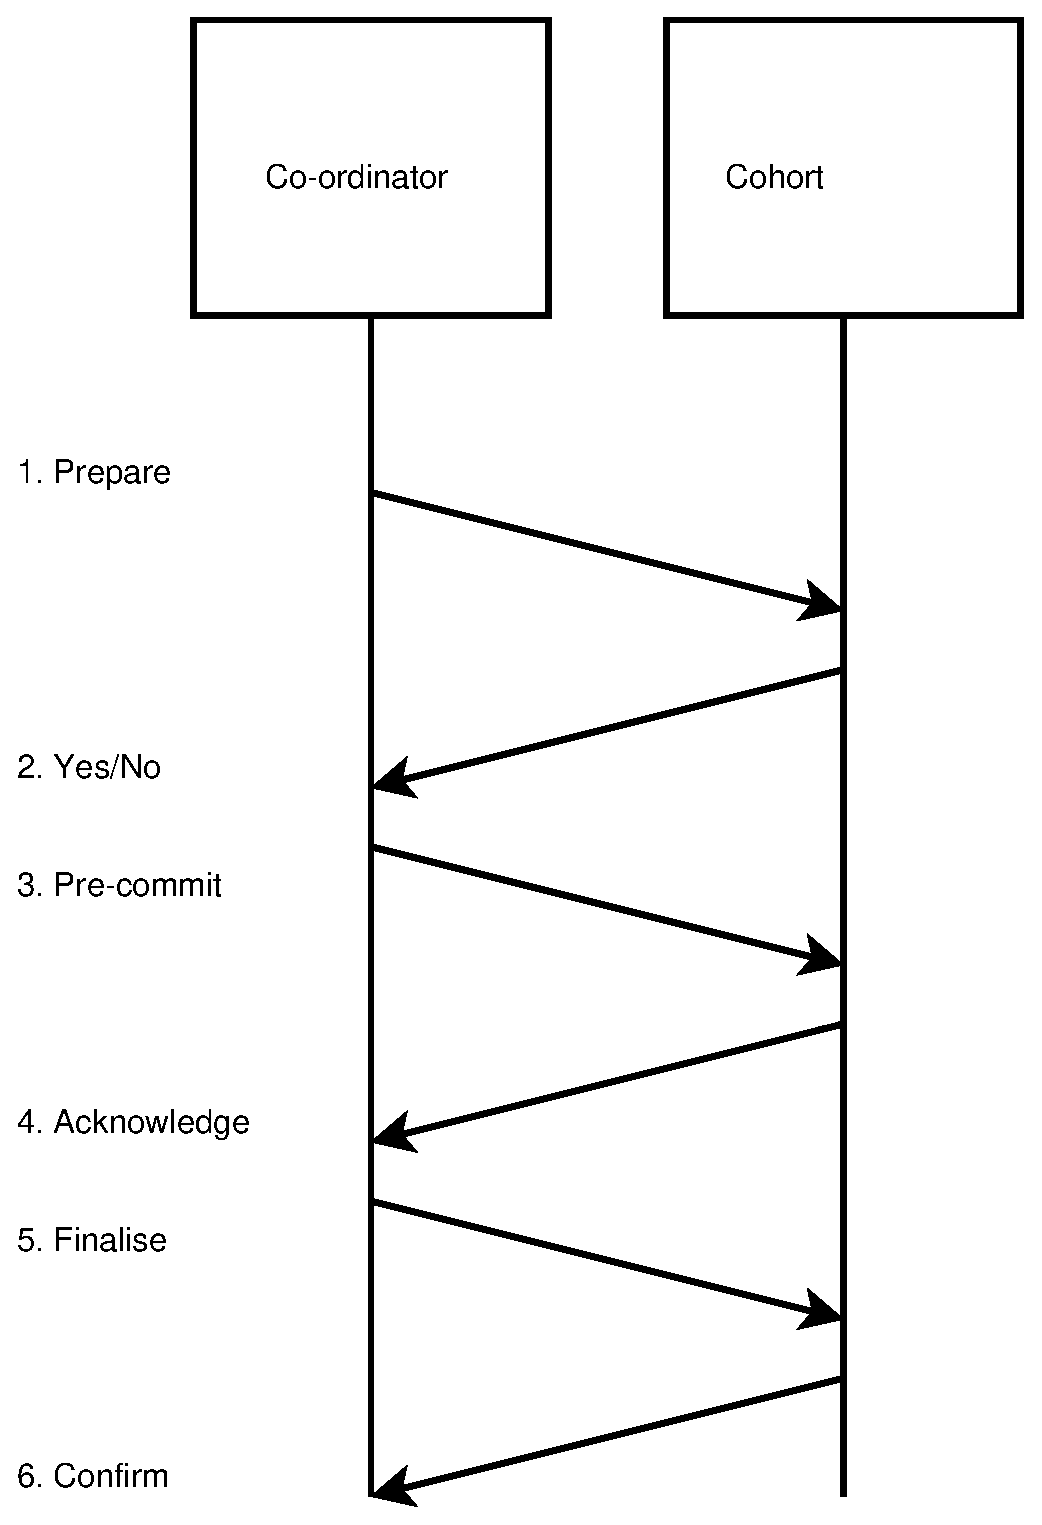
\includegraphics[scale=0.5]{figs/three-pc.eps}
\caption{\label{fig:three-pc}Three Phase Commit}
\end{figure}

3 Phase Commit (3PC) is a modification of 2PC that turns it from a synchronous protocol into an
asynchronous protocol. This is done by adding a third phase, so that we can use timeouts to assert
the state of the system at any point in time. Again the basic message flow is shown in
figure~\ref{fig:three-pc}. The three phases are:

\begin{enumerate}
\item \msg{Prepare}: the co-ordinator asks the cohort members if they can perform the operation. At
	this stage if there is a failure or timeout, the co-ordinator aborts the transaction.
\item The cohort respond with a \msg{YES} or \msg{NO}. Again, if there is a failure or timeout the cohort
	member considers the transaction aborted.
\item \msg{Pre-commit}: If the co-ordinator receives \msg{YES} messages from every member of the
	cohort, it sends a \msg{Pre-commit} message to them all, otherwise it aborts the
	transaction. It also aborts in the case of a failure or timeout.
\item \msg{Acknowledge}: If the cohort member receives a \msg{Pre-commit} message, it replies with
	an \msg{Acknowledge} message. If the co-ordinator aborts, or there is a failure or
	timeout, the cohort member aborts.
\item \msg{Finalise}: If the co-ordinator times out, it aborts the transaction. Otherwise, when it
	has received \msg{Acknowledge} messages from every cohort member it sends a \msg{Finalise}
	message to them all.
\item \msg{Confirm}: Once a cohort member has received a \msg{Finalise} message, it commits the
	transaction, even if the co-ordinator fails. It can reply with a \msg{Confirm} message.
\end{enumerate}

This fixes the problem of node failure, but still suffers from a significant problem. If there is
a network partition, and all nodes who voted \msg{YES} are in one half and all nodes who voted
\msg{NO} are in the other, both partitions will recover into different, inconsistent states.
Brewer's CAP theorem \cite{gilbert2002} says that we cannot achieve both consensus and availability
during a network partition - we must choose one. 3PC opts for availability, but for a distributed
database with ACID properties it is preferable to have consensus. Paxos guarantees consensus at
the cost of lack of availability in a network partition.

\section{Paxos}

\subsection{Introduction}

Paxos is a distributed consensus algorithm. It was developed by Leslie Lamport at Microsoft
research when he was trying to disprove its existence. Paxos is failure tolerant for up to $F$
simultaneous failures in a network of $2F + 1$ nodes.
% S comment: Explain why this is true (ie, showing some working)

Paxos is actually a family of protocols, based around the same main algorithm. The Paxos algorithm
is an algorithm for agreeing on a single value across a network of processors. Paxos has several
safety and liveness properties:

\paragraph{Safety Guarantees}

\begin{itemize}
\item Integrity - every correct process decides at most one value, and if it decides some value v,
	then v must have been proposed by some process.
\item Agreement - Every correct process must agree on the same value.
\item Non-triviality - Only a value that has been proposed can be chosen.
\end{itemize}

% Consistency
%     At most one value can be learned (i.e., two different learners cannot learn different values).[8][9]
% Only a single value is chosen
%
% Liveness(C;L)
%     If value C has been proposed, then eventually learner L will learn some value (if sufficient processors remain non-faulty).[9]
%
%
% A process never learns that a value has been chosen unless it has been

\paragraph{Liveness Properties}

\begin{itemize}
\item Some proposed value is eventually chosen
\item If a value is chosen, a process eventually learns it
\item Termination - Every correct process decides some value.
\end{itemize}

% \begin{enumerate}
% 	\item Consistency: Only one value is chosen.
% % XXX: wtf, how can we guarantee liveness, yet liveness is impossible??
% 	\item Liveness: If a value is proposed, eventually some value is chosen.
% 	\item Non-triviality: only proposed values may be chosen.
% \end{enumerate}

Paxos can tolerate certain kinds of failures. These are: messages being lost, delayed, repeated or
delivered out of order. It is correct even with multiple leaders, and will reach consensus if
there is a single leader that talks to a majority of processes twice.

% Paxos can tolerate lost messages, delayed messages, repeated messages, and
% messages delivered out of order. It will reach consensus if there is a single
% leader for long enough that the leader can talk to a majority of processes
% twice. Any process, including leaders, can fail and restart; in fact all
% processes can fail at the same time, the algorithm is still safe. There can be
% more than one leader at a time.
%
% Paxos is an asynchronous algorithm; there are no explicit timeouts. However, it
% only reaches consensus when the system is behaving in a synchronous way, ie
% messages are delivered in a bounded period of time; otherwise it is safe. There
% is a pathological case where Paxos will not reach consensus, in accordance to
% FLP, but this scenario is relatively easy to avoid in practice.

However Paxos cannot tolerate ``rogue'' processes, that is, processes deliberately sending
malicious or incorrect messages. There is a variant of Paxos called \emph{Byzantine Paxos} which
can tolerate this, albeit at a failure tolerance of $F$ for $3F + 1$ nodes. I will not go into
this variant further in this dissertation.

\subsection{Definitions}

\subsubsection*{Proposals}

In an instance of Paxos, values that can be accepted are called \emph{proposals}. A proposal is a
2-tuple of the form ($n$, $v$), where $n$ is the unique proposal number and $v$ is the value
proposed.

\subsubsection*{Proposal Numbering}

One of the assumptions that Paxos makes is that every proposal has a unique proposal number. This
is necessary so that proposals have a \emph{total order}. A total order means that every proposal
can be compared to any other proposal. This is necessary in order to
find the maximum ordered proposal. The conventional way to achieve this is to define a proposal
number as a 2-tuple of (sequence number, node address). These can be compared lexicographically,
and as node addresses are unique, every proposal number will be unique. In practice I plan to use
UUIDs as node identifiers, in order to be confident of their uniqueness.


\subsubsection*{Messages}

Paxos utilises several message types:

\begin{itemize}
\item \msg{Prepare(n)}, asking the recipient to respond with a \msg{Promise} not to
	accept any proposals numbered less than $n$.
\item \msg{Promise(n, m, v)}, promising to only accept proposals numbered greater than or equal to
	$n$. $m$ refers to the number of the highest proposal previously accepted by the recipient and
	$v$ is the value of that proposal. If they are not included and the message is in the form
	\msg{Promise(n)}, it is assumed that the recipient has not accepted any proposals
		previously.
\item \msg{AcceptRequest(n, v)}, asking the recipient to accept the proposal ($n$, $v$).
\item \msg{AcceptNotify(n, v)}, notifying the recipient that the sender has accepted the proposal
	($n$, $v$).
\end{itemize}

\subsection{How it works}

\label{sec:how-paxos-works}

The central concept of Paxos is that of majority vote. A \emph{quorum} is defined as a majority of
nodes in the system.  Paxos requires a quorum of nodes to accept a proposal before the proposal is
considered ``learnt'' by the network. As any quorum of nodes must share at least one node with any
other quorum, if a proposal is accepted by a quorum $Q$ and learnt, any subsequent decision taken
must involve at least one node $q \in Q$.

Paxos is comprised of two stages. First, a quorum of nodes $Q$ are sent \msg{Prepare} messages to
prepare them to accept a proposal. They respond with the greatest proposal they have previously
accepted. It is this key step which ensures that Paxos enforces consistency. In the second step,
the co-ordinating node sends out a proposal for nodes to accept. However, the value of this
proposal must be the value of the greatest proposal previously accepted by a node in $Q$.

\subsubsection*{Formal description of the algorithm}
In \emph{Paxos Made Simple} \cite{lamport01}, the actions of a Paxos node are split into three
roles - Proposer, Acceptor and Learner. Explaining it in terms of these roles is simpler, however
in practice they are combined into one client.

\subsubsection*{Proposer}

\paragraph{Phase 1}

To start a round of Paxos, the Proposer $P$ sends out a \msg{Prepare(n)} message to the acceptors in
the network with a unique proposal number, $n$. This proposal number $n$ must
be higher than any proposal numbers $P$ has sent for this instance of Paxos.

\paragraph{Phase 2}

If the Proposer receives  replies from a quorum of acceptors, $Q$,
to its \msg{Prepare(n)} message, it sends the message \msg{AcceptRequest(n, v)} to all
$q \in Q$, where $v$ is defined as follows. If the message set $M$ is defined as
${(n, v) for all \msg{Promise(n, v)}}$, $v$ is defined as
$(n', v) \in M. \forall (n'', v'') \in M.  n' >= n''$.
Informally, $v$ the value of the maximum \msg{Promise(n, v)} received.

\subsubsection*{Acceptor}

Acceptors need to store a few variables. An acceptor $A$ stores:
\begin{itemize}
\item $\rho$ - the greatest proposal number that $A$ has received in a \msg{Prepare} message and
	responded to with a \msg{Promise} message.
\item $\eta$ - the highest-numbered proposal $A$ has accepted (initialised to $0$).
\item $\nu$ - the value of proposal $\eta$ (initialised to \verb+null+).
\end{itemize}

\paragraph{Phase 1}

If an Acceptor $A$ receives a message \msg{Prepare(n)}, and $n > \rho$, then it replies with the
message \msg{Promise(n, $\bm{\eta}$, $\bm{\nu}$)} and sets $\rho$ to $n$. This means it will not
accept any proposals numbered less than $n$. If it has not accepted any proposals yet then $\eta$
and $\nu$ will still be set to their initial values.
% XXX

\paragraph{Phase 2}

If an Acceptor receives a message \msg{AcceptRequest(n, v)}, if $n > \rho$ it accepts the
proposal, setting $\eta := n$ and $\nu := v$. It also notifies Learners in the network of its
decision by sending an \msg{AcceptNotify(n, v)} message to them.

% % XXX: is this PMS or PTP??
% \emph{Paxos Made Simple} \cite{lamport01} describes several different ways of notifying Learners
% of accepted proposals. One way is to specify a \emph{distinguished Learner}, who then notifies
% other Learners when a quorum of Acceptors has accepted a proposal. This can also be extended to specify several
% distinguished Learners. or we can broadcast all \msg{AcceptRequest} messages to all Learners.
% While this method generates $L\times A$ messages (where $L$ is the number of Learners in the
% network and $A$ is the number of Acceptors in the network), it is the simplest and the most
% resilient to failures, and therefore the one I have chosen to implement. By contrast, the first
% method generates $A + L$ messages, and the second generates $D\times A + L$ messages, where $D$ is
% the size of the set of distinguished Learners.

\subsubsection*{Learner}

% XXX: pseudo code?
Learners must store a map of proposal numbers $\rightarrow$ acceptor IDs. When a Learner receives a
message \msg{AcceptNotify(n, v)} from an Acceptor $A$, it must add $A$ to the set of Acceptors who
have accepted proposal $n$. When this set becomes a quorum (ie, the size of the set $S$ becomes
greater than $N / 2$, where $N$ is the size of the network), the Learner can ``learn'' the $v$ as
the value decided on for that instance of Paxos. Because of the properties of Paxos, once a quorum
of acceptors has accepted the proposal ($n$, $v$), the value of that instance will never change.

\subsection*{Examples}

The behaviour of Paxos is perhaps best explained with a few examples of different situations.

\subsubsection*{Normal Behaviour}

\begin{figure}[h!]
\centering
\lwincludegraphics{figs/paxos-msg-flow-usual.eps}
\caption{\label{fig:paxos-usual}Paxos Message Flow: Usual Behaviour}
\end{figure}

Figure~\ref{fig:paxos-usual} shows the message flow for a
complete round of Paxos if there are no failures and everything proceeds as expected. In this
case, then the behaviour is reasonably straightforward to follow. There are four message delays
until the proposed value is learnt.

\begin{enumerate}
\item \msg{Prepare(n):} The Proposer sends a \msg{Prepare} message to the Acceptors.
\item \msg{Promise(n):} The Acceptors all promise to accept proposals numbered $>= n$, as they
	have not seen any \msg{Prepare} requests yet and therefore trivially cannot have promised
	to accept a proposal higher than $n$.
\item \msg{AcceptRequest(n, v):} The Proposer sends a value $v$, with the proposal number $n$, to
	the Acceptors.
\item \msg{AcceptNotify(n, v):} The Acceptors have not made any promises preventing them from
	accepting $n$, so they accept $v$ as the value for the round of Paxos and notify the
	Learner.
\end{enumerate}

\subsubsection*{Acceptor Failure}

\begin{figure}[h!]
\centering
\lwincludegraphics{figs/paxos-msg-flow-one-acceptor-fail.eps}
\caption{\label{fig:paxos-acceptor-fail}Paxos Message Flow: Acceptor Failure}
\end{figure}

Figure~\ref{fig:paxos-acceptor-fail} shows the same
scenario, but with a single Acceptor failing. In this case there is still a quorum of Acceptors
available, so behaviour carries on as normal. There are still four message delays until the
proposed value is learnt.

\begin{enumerate}
\item \msg{Prepare(n):} The Proposer sends a \msg{Prepare} message to the Acceptors.
\item Failure: Acceptor 3 fails.
\item \msg{Promise(n):} Acceptors 1 and 2 still promise to accept the proposal, for the same
	reason as before.
\item \msg{AcceptRequest(n, v):} The quorum size is 2, so a quorum of acceptors has responded, and
	the Proposer can continue as normal.
\item \msg{AcceptNotify(n, v):} The Learner receives \msg{AcceptNotify} messages from a quorum of
	Acceptors, so also continues as normal, learning the value $v$.
\end{enumerate}

\subsubsection*{Partition}

\begin{figure}[h!]
\centering
\lwincludegraphics{figs/paxos-msg-flow-partition.eps}
\caption{\label{fig:paxos-partition}Paxos Message Flow: Partition}
\end{figure}

% This is to get this figure on the next full page, ie *before* the duelling section rather than
% on a random page after it...
\begin{figure}[p]
\centering
\lwincludegraphics{figs/paxos-msg-flow-duelling.eps}
\caption{\label{fig:paxos-duelling}Paxos Message Flow: Duelling Proposers}
\end{figure}

Figure~\ref{fig:paxos-partition} shows what happens in a
network partition. A second Proposer is able to continue the instance of Paxos, and no
inconsistencies are allowed to occur in the network, as the left half of the partition is unable
to make progress until the partition is resolved, at which point it can learn the decisions made
by the half of the partition that was able to make progress.

\begin{enumerate}
\item \msg{Prepare(1):} The Proposer sends a \msg{Prepare} message to the Acceptors, but is only
	able to successfully message one of them.
\item \msg{Prepare(2):} A second Proposer simultaneously sends a \msg{Prepare} message to the
	Acceptors, and is able to reach a quorum.
\item \msg{Promise(1):} The Acceptor on the left side of the split replies with a \msg{Promise},
	but does not make up a quorum.
\item the first Proposer times out. It could restart with a higher proposal number, but in this
	case it will be unable to make any progress until the partition is resolved.
\item \msg{Promise(2):} The Acceptors on the right side of the split both reply with a
	\msg{Promise}, making a quorum.
\item \msg{AcceptRequest(2, b):} The second Proposer asks the Acceptors to accept 'b' as the
	value.
\item \msg{AcceptNotify(2, b):} The Acceptors make up a quorum so are able to proceed through to
	completion.
\end{enumerate}

\subsubsection*{Duelling Proposers}

Figure~\ref{fig:paxos-duelling} shows the worst case scenario
for Paxos -- duelling Proposers. This is the pathological case for Paxos where it is possible for
it to never make progress. However this eventuality is unlikely because the messages from the proposers
must interleave so that there is no contiguous sequence of \msg{Prepare} and \msg{AcceptRequest}
messages. This means that if any single Proposer manages to send a \msg{Prepare} message followed by a
subsequent \msg{AcceptRequest} message to a quorum of Acceptors, consensus will be achieved.

\begin{enumerate}
\item \msg{Prepare(1):} The Proposer sends a \msg{Prepare} message to the Acceptors as usual.
\item \msg{Prepare(1):} The Acceptors respond with a \msg{Promise} to only accept proposals
	numbered $>= 1$.
\item \msg{Prepare(2):} Before the first Proposer sends an \msg{AcceptRequest} message, another
	Proposer sends a \msg{Prepare} message to the Acceptors asking them to only accept
	proposals $>= 2$.
\item \msg{Promise(2):} The Acceptors promise to do so.
\item \msg{AcceptRequest(1, a):} The first Proposer sends an \msg{AcceptRequest} message to the
	Acceptors, but they cannot accept as they have promised to only accept proposals $>= 2$.
\item \msg{Nack(2):} The Acceptors inform the Proposer they cannot accept with a \msg{Nack}
	message. This step is not strictly necessary as the Proposer would retry with a higher
	proposal number after a timeout, but is included for clarity.
\item \msg{Prepare(3):} The Proposer sends another \msg{Prepare} message to the Acceptors...
\item \msg{Promise(3):} and they promise not to accept proposals $>= 3$
\end{enumerate}

% XXX
This cycle can continue indefinitely, but the probability of it doing so becomes very small very
quickly.

\subsection{MultiPaxos}

While Paxos is capable of forming consensus in a single network, it can only agree on a single
value. A distributed application needs a series of values rather than a single value. There are
several ways to achieve this. The way outlined in \emph{Paxos Made Simple} \cite{lamport01}, known
as MultiPaxos, is by a form of leader election. The Proposer who proposed the successful value in
the last round of Paxos becomes the leader, and is only required to send a \msg{AcceptRequest}
message in the subsequent instance to have a value accepted -- by winning the last round there is
an implicit Phase 1. If this \msg{AcceptRequest} fails for whatever reason, the instance degrades
into a standard instance of Paxos.

In my project I chose an even simpler approach to running multiple rounds of Paxos. Each instance
of Paxos runs independently in my application, unaware of any other instance. This is a simple and
effective way of having multiple instances of Paxos running, although it does have drawbacks,
which I will go into in my evaluation chapter.


\cleardoublepage
\chapter{Implementation}

\section{Event Driven Programming}

Event Driven Programming is a paradigm that involves structuring the program flow around events
that occur. For a distributed application this mainly means in response to network packets
arriving, but can also be caused by user input or by timers firing. Program flow is co-ordinated
by an event loop, which calls appropriate callbacks when events occur. When the event is handled,
execution yields to the event loop again, which handles the next event. This means the code is not
concurrent and does not need to be thread safe, which makes reasoning about it a lot simpler.
Twisted provides the event loop and network interfaces, so it is relatively trivial to listen on
an interface and have a callback be passed events that occur.

A useful class that Twisted provides is the Deferred class. This represents the ``promise'' of a
value which has not actually been learnt yet. It can be passed around in place of the value, and
callbacks added to it in a chain that will be called when the value is finally learnt.

\section{Module Design}

\begin{figure}[htb]
\centering
\lwincludegraphics[scale=0.5]{figs/module-layout.eps}
\caption{\label{fig:module-layout}Simplified module layout}
\end{figure}

Figure~\ref{fig:module-layout} shows the basic design for the code, illustrated with how objects
are passed through the different layers. The DBP Core class is the main event handler, passing
operations down to Paxos through the Manager class to be committed to the network. The Manager
class receives operations from Paxos in the order they are learnt. It then passes operations up to
the DBP Core class in order, as they become available. An operation is available if the operation
that precedes it has been received, ie, every operation before it is also available. The DBP Core
class then interfaces with the database, which is a simple row-based table.

\section{Paxos Design}

\subsection{Protocol Design}

As I found initially found the concept of Paxos and how it works reasonably confusing, and wasn't
sure how to implement in code various concepts outlined in the academic papers I read (mainly
\emph{Paxos Made Simple} \cite{lamport01}), I wanted to iterate from one prototype of the protocol
to another quickly, adding features as I began to understood how the protocol worked better.

My initial prototype was a synchronous model that sent messages internally. I quickly decided to
change to Twisted, as I hoped the support it would give me would make writing the protocol easier.

\subsubsection*{Messages}

\label{sec:message-serialization}

I initially decided to use a class hierarchy to define messages, and to use a simple
serialization/deserialization technique, transmitting messages in the form
\verb+"<message type>":<proposal serialization>+. I decided to send messages as simple strings
over the network for a number of reasons - for a prototype implementation speed was not my primary
concern, iterating towards the most complete and correct solution in a reasonable period of time
was. Furthermore, even if my priority was speed, optimising the message format felt like a
premature optimisation, and using a binary format would vastly hinder my debugging.

In hindsight restricting messages to only a combination of message type and proposal attributes
was unnecessarily restrictive. An advantage of constructing them in this way was to prevent typos
in creating messages (cf. \verb+send(Msg({"msg_type": "accept_requst", ...}))+
and \verb+send(Msg({"msg_type": "accept_request", ...}))+).

Although security was not a major concern for this project, I wanted to be able to serialize
arbitrary objects without allowing remote code execution on a host running my software - even
though it was only running on local host this still seemed unnecessarily risky. Fortunately Python
has a builtin function called \verb+literal_eval+ which only evaluates literals (strings, tuples,
lists and dictionaries), and nothing unsafe (classes, functions) which could be used to run
arbitrary code.

I eventually moved to sending a dictionary in plain string format over the network. This allowed
me to specify arbitrary key/value pairs without having to add in extra support for them (a
limitation I initially struggled with before moving to this format). This greatly simplified a lot
of logic, at the cost of trusting that messages received are well formed.  However, this is not
too problematic for several reasons - firstly, if the message is not well formed, the code will
throw an exception, which will be caught by the message handler and discarded. Paxos allows for
any message to be ignored or dropped and still guarantees correctness (it must do this in order to
work if a packet is dropped in the network or delayed indefinitely). If correctness of the message
needed to be verified, it would be relatively easy to add a checksum of some kind, a very simple
form of this is found in the \emph{netstring} format (defined by DJB at
\verb+http://cr.yp.to/proto/netstrings.txt+). This is easily added to my classes by making them
inherit from \verb+NetstringReceiver+ rather than \verb+DatagramProtocol+, and using
the \verb+stringReceived+ callback rather than the \verb+datagramReceived+ callback. In any case,
it is beyond the scope of this project to deal with malicious nodes, so I did not spend a
significant amount of time considering this problem.

\subsubsection*{Hosts}

I first used a tuple of \verb+(IP Address, Port Num)+ to identify hosts. However there turned out
to be a number of problems with this. Firstly as an identifying scheme it is not persistent across
interfaces. Also there is a significant problem if a node needs to identify itself (a pertinent
example is for the \op{ATTEMPTLOCK} operation). After I changed the message format to a generic
dictionary format, I wanted to add an attribute specifying the sender. This is difficult to do
using tuple format, as it is non-trivial for a host to obtain its own IP address, it may be on a
local network or behind a NAT for example.

For this reason, I updated the code to use a \emph{globally unique identifier} (GUID). This is
better than using a tuple for the reasons identified above - the host is now aware of its own
address and is able to include it in messages, and there are no problems in potentially ambiguous
adapter situations, where different parts of the network think a node has different addresses.

There is the problem of a node lying about its identity, for example forging a \op{ATTEMPTLOCK}
request. This is a more pertinent problem because I am using UDP, which is easier to forge than
TCP. Although a fully secure implementation is beyond the scope of this project, one potential
solution would be to sign or authenticate messages, and include this signature or MAC with the
message.


\subsection{Protocol Extras}

On top of the basic Paxos protocol I added some extra features to the protocol, in particular,
node discovery and bootstrap; and heartbeat monitoring of nodes to detect them leaving the
network.

Keeping an accurate idea of network membership is a key requirement of Paxos. Each node in the
network needs to have a good idea of the number of nodes in the network in order to have an
accurate estimate of the quorum size. If a node underestimates the quorum size, the network may
become inconsistent, as a node may ``learn'' a value erroneously. On the other hand, if we
overestimate the quorum size, we may not make any progress, waiting for more responses than there
are nodes in the network. In practice, the first problem is more problematic than the second,
which is only temporary - as long as the node eventually accurately learns the quorum size the
network will make progress, however if the network develops inconsistencies these are much harder
to resolve.

% Consensus algorithms need a strong failure detector \cite{chandra96}.

\subsubsection{Bootstrap}

A node connects to the network by connecting to a \emph{bootstrap node}. In my current
architecture this can be any node, however in a different model it may be a specific node, see the
Evaluation chapter for more details involving scaling. When a node $N$ connects to the bootstrap
node $B$, it sends an \msg{EHLO} message. $B$ replies with a \msg{Notify} message containing all the
hosts $B$ is aware of. $N$ then sends each of these in turn \msg{EHLO} message, making each of them
aware of its presence, and getting a \msg{Notify} message from each othem. This is repeated until
there are no nodes it has not learned of. $N$ is then fully integrated into the network.

Note that this bootstrap method is $N^2$ in the number of messages sent. There are other ways to
do bootstrap that are more efficient in the number of messages sent (for instance a DHT or a
supernode hierarchy). While this architecture is out of the scope of this project these options are
discussed later on.

\subsubsection{Heartbeat}

In order to identify when a node leaves the network, when a node initialises it starts a timer on
a configurable timeout and sends a \msg{Ping} message to every node in its \verb+hosts+ attribute.
It then copies the \verb+hosts+ set to a \verb+timeout_hosts+ set. As it receives a reply from a
host it removes that host from the \verb+timeout_hosts+ set. When the timeout fires, any nodes who
have not sent a \msg{Pong} in reply are left in the \verb+timeout_hosts+ set, and are removed from
the \verb+hosts+ set.

\subsection{MultiPaxos}

The simple way MultiPaxos is implemented is multiple instances of Paxos operating in parallel.
Paxos is implemented as a state machine, with the instance state as a Python dictionary and
transitions as methods. A simple way to implement MultiPaxos is to have every transition method
take an instance dictionary as an argument and operate on that. One problem with this approach is
that if any initial messages (\msg{Prepare}, \msg{AcceptRequest}, etc) are not received, the
initial state is not constructed.

For certain messages that are not linked to any particular instance of Paxos, the message
attribute \verb+"instance_id"+ is sent with value \verb+None+, for all other messages the instance
id is an integer referring to the OID of the instance of Paxos running. For example, all messages
corresponding to OID 2 in the operation log would have the attribute \verb+"instance_id": 2+ set
in their message dictionary.

\subsection{Implementing NACKS}

Paxos is designed to be preserve its safety and liveness properties even when messages are dropped
or lost. In order to account for messages being lost, the algorithm must retry when there is a
timeout (see explanation of Proposer mixin). This is done with timeouts. In fact, the simplest
implementation of Paxos uses ignored packets to communicate between nodes - if a message doesn't
\emph{require} a response it just ignores it.

An example where this happens in cases such as if an Acceptor $A$ has accepted a proposal
$\mathcal{P}_1$ from Proposer $p_1$, with a proposal number of $\varphi_1$. $A$ then receives a
\msg{Prepare} message $M$ from Proposer $p_2$. $M$ has proposal $\mathcal{P}_2$, such that
$\mathcal{P}_2$ has proposal number $\varphi_2$ and $\varphi_1 > \varphi_2$. In my original
implementation of Paxos, $A$ would simply drop the message $M$, and leave it until the timeout $t$
for $p_2$ to resend $M$ with a higher proposal number. This has the significant disadvantage that
if $p_1$ has crashed, $p_2$ must go through $\varphi_2 - \varphi_1$ messages, and $t\times
(\varphi_2 - \varphi_1)$ seconds before it gets a response ($p_2$ will know $A$ still exists
because it will still respond to \msg{PING} messages).

% XXX split this into NACK, and NACK + p_2

A faster method is to introduce a new message type \msg{NACK}. If $A$ sends $p_2$ a \msg{NACK}
message containing the $\varphi_2$, $p_2$ can update its current proposal number to $\varphi_2 +
1$, and not even have to wait for one timeout period before receiving a \msg{Promise} message. A
disadvantage of this extension to the protocol is that it can increase the probability of duelling
proposers, and therefore increase the latency of the protocol. I shall discuss this in my
evaluation.

However, this still exhibits ``ping pong'' behaviour, with \msg{NACK}s and \msg{Prepare}s bouncing
between Proposer and Acceptor until the Proposer catches up with the Acceptor. We can remove this
message bounce by adding information to the \msg{NACK} message specifying the proposal number the
Acceptor has accepted, allowing the Proposer to update the proposal number it tries immediately.
This is ``NACK version 2''.

% can speed up even further by adding information (correct answer)

With either of these versions of the extension, the protocol still has protection from dropped or
lost messages (the safety and liveness properties are still preserved), but in the case of a
crashed Proposer, the recovery should be far quicker.

\section{Paxos Implementation}

\subsection{Node}

The \verb+Node+ class is the manager class for a Paxos node, and co-ordinates between the three
role mixins. It handles message dispatch and instance handling as explained below, as well as
managing the quorum size, which needs to be managed accurately for decisions made by both the
Proposer and Learner roles, through heartbeat and network discovery.

\subsubsection{Message Dispatch}

As mentioned in Section~\ref{sec:how-paxos-works}, the actions of a node can be split into three
roles. I implemented Paxos by splitting the responsibilities into the three roles. I then made a
handler class for each role that only implemented the functionality required for that role
(\verb+Proposer+, \verb+Acceptor+, \verb+Learner+). Each class implements methods to handle a
message type. The \verb+Node+ class then inherits from all three mixin classes, and delegates to
each of them as appropriate. It does this by checking the \verb+msg_type+ attribute on a message,
and then looking up a method called \verb+recv_<msg_type>+ on itself.

For example, the \verb+Proposer+ class implements the \verb+recv_prepare+ method. When a node
receives a \msg{Prepare} message, the \verb+msg_type+ attribute is set to \verb+"prepare"+. The
\verb+datagramReceived+ callback is called by Twisted with the datagram as a string. The method
parses the string serialization into a dictionary (as described in
Section~\ref{sec:message-serialization}), checks the \verb+msg_type+ attribute, which is
\verb+prepare+. It then looks up the \verb+"recv_prepare"+ method on itself, which is implemented
by the \verb+Proposer+ subclass. It then calls \verb+self.recv_prepare+, passing in the message,
and also the Paxos instance dictionary (described in section~\ref{sec:paxos-instance}). If an
message is received with an unknown message type it is dropped, and a message is logged.

Once the instance's status is set to \verb+complete+, all messages for this instance are dropped -
this prevents delayed messages restarting or affecting completed instances.

Below is a table outlining which message types are delegated to which mixin classes. \\

\begin{tabular}{ | c | c | p{7cm} | }
  \hline
  {\bf Message type} & {\bf Handler Class} & {\bf Message action} \\ \hline
  AcceptRequest & Acceptor & Respond with AcceptNotify (if valid) and accept Proposal. \\ \hline
  AcceptNotify & Learner & Record response and if a quorum has accepted that proposal, learn it. \\ \hline
  EHLO & Node & Respond with notify. \\ \hline
  Notify & Node & Add hosts to host list. \\ \hline
  Ping & Node & Send pong.  \\ \hline
  Pong & Node & Remove host from timeout list. \\ \hline
  Prepare & Acceptor & Respond with Promise (if valid). \\ \hline
  Promise & Proposer & Respond with AcceptRequest and deal with timeouts. \\ \hline
\end{tabular}

\subsubsection{Instance Handling}

\label{sec:paxos-instance}

As noted in the previous section, message handlers are called with the message to be handled, but
also with an instance dictionary with state information of the current instance of Paxos running.
If the node running initiated the instance of Paxos, then when it initiated the instance it will
have created an instance dictionary, but otherwise the first the node knows about the instance is
when it receives the first message about it (likely to be a \msg{Prepare} message, but may not be
due to dropped messages or not being include in the quorum of Acceptors).

When this happens, the datagram callback detects that the node has not encountered any instances
with that instance ID before, and creates a new instance, storing it in the instance dictionary.
To create a new instance state dictionary, it calls the \verb+create_instance+ method, which
creates a new instance state. This contains a callback to be fired when a value is learnt for that
instance of Paxos, and then calls a method from each of the three mixin classes, so they can add
any variables that class uses to the instance state. This keeps knowledge of how each role is
implemented encapsulated in the mixin class.

\subsection{Role Mixins}

\subsubsection{Proposer}

% XXX: Should this be psuedo code?
% XXX: state diagram
% XXX: variables saved in instance state?

\begin{tabular}{ | c | p{7cm} | }
  \hline
  {\bf Variable} & {\bf Usage} \\ \hline
  \verb+quorum+ & set of GUIDs of Acceptors accepting the current proposal \\ \hline
  \verb+status+ & current state of the state machine \\ \hline
  \verb+last_tried+ & last proposal number \\ \hline
  \verb+restart+ & restart boolean \\ \hline
  \verb+proposer_prev_prop_num+ & highest proposal number accepted by any acceptor in \verb+quorum+ \\ \hline
  \verb+proposer_prev_prop_value+  & value corresponding to \verb+proposer_prev_prop_num+ \\ \hline
\end{tabular}


The Proposer mixin is the most complicated out of the three roles. It is a simple state
machine with 3 states: ``idle'', ``trying'' and ``polling''. The Proposer initialises the state to
the ``idle'' state. It then transitions to the ``trying'' state and sends \msg{Prepare} messages
with a proposal number \verb+(p, <GUID>)+, where $p$ is normally 1, but may be different if we
have reached the ``trying'' state from the timeout handler (described below). The \msg{Prepare}
messages are sent to the Acceptors in the network which in my design is any node, as any node in
the network can act as an Acceptor because the network is homogenous. It also stores the proposal
number in the instance dictionary. It then schedules a timer to fire after the timeout period,
which is specified in a configuration module.

When the timer fires, Twisted will call the timeout function, \verb+handle_proposer_timeout+. We
can specify the arguments we want Twisted to call \verb+handle_proposer_timeout+ with when we
schedule the timer. \verb+handle_proposer_timeout+ is called with the instance state and the
current state of the state machine. \verb+handle_proposer_timeout+ first checks if the Proposer is
in this state, and if not, it does nothing. So if the Proposer has not transitioned into another
state by the time the timeout fires, the timeout handler will retry the ``trying'' stage, with a
higher proposal number. If the proposal number stored in the instance dictionary is of the form
\verb+(p, <GUID>)+, the handler will retry with proposal number \verb$(p+1, <GUID>)$. It does this
by calling \verb+proposer_start+ with the new proposal number.

When the Proposer is in the ``trying'' state, it receives \msg{Promise} messages. If the proposal
number is not the same as the proposal sent out most recently, this means the Acceptor has
promised to accept a proposal we are no longer interested in. We can check the proposal number of
the message against the \verb+last_tried+ state variable and if they are not the same then the
message is dropped.

As the Proposer receives \msg{Promise} messages, it keeps track of the \verb+prev_prop_num+ and
\verb+prev_prop_value+ attributes of messages it has received. If \verb+prev_prop_num+ is larger
than \verb+proposer_prev_prop_num+, then it updates \verb+proposer_prev_prop_num+
and \verb+proposer_prev_prop_value+ to \verb+prev_prop_num+ and \verb+prev_prop_value+
respectively.

Once a Proposer in the ``trying'' state has received \msg{Promise} messages from a majority of
Acceptors in the network, it moves to the ``polling'' state. The Proposer examines the responses
from the Acceptors and finds the highest numbered proposal that has been accepted by an Acceptor
in the quorum. It then sends \msg{AcceptRequest} messages containing the value $v$ that is
associated with that proposal. If there is no proposal that has been accepted by an Acceptor in
the quorum then the Proposer is free to set its own value for that instance. This means that if
the Proposer has been directed to set a value $v_1$ and is forced by the protocol to set a
different value $v_2$, as $v_2$ has already been accepted by a node in the network, it starts a
new instance of Paxos with $v_1$ as the value, to ensure $v_1$ is eventually committed to the
network. This restart may be skipped if we are merely ``chasing up'' a value, ie there is a gap in
the operation log and we need to ascertain the value.


\begin{figure}[htb]
\centering
\lwincludegraphics[scale=0.5]{figs/proposer-state-machine.eps}
\caption{\label{fig:proposer-state-machine}Proposer State Machine}
\end{figure}

\subsubsection{Acceptor}

The Acceptor role is a fairly simple class that only stores three variables in each instance:

\begin{tabular}{ | c | p{7cm} | }
  \hline
  {\bf Variable} & {\bf Usage} \\ \hline
  \verb+acceptor_prepare_prop_num+ & The highest Proposal number we have seen - corresponds to
  $\rho$ \\ \hline
  \verb+acceptor_cur_prop_num+ & The current accepted Proposal - $\eta$ \\ \hline
  \verb+acceptor_cur_prop_value+ & The value of Proposal $\eta$, corresponds to $\nu$ \\ \hline
\end{tabular}

The implementation is a near-direct version of the description of the algorithm in the Preparation
section.

When an acceptor receives a \msg{Prepare(n)} if $n > $
If an acceptor $A$ receives a message , and $n > \rho$, then it replies with the
message \msg{Promise(n, $\bm{\eta}$, $\bm{\nu}$)}, meaning that it will not accept any proposals
numbered less than $n$.

\paragraph{Phase 2}

If an acceptor receives a message \msg{AcceptRequest(n, v)}, if $n > \rho$ it accepts the
proposal, settings $\eta := n$ and $\nu := v$. It also notifies Learners in the network of its
decision by sending an \msg{AcceptNotify(n, v)} message to them.

% XXX: is this PMS or PTP??
\emph{Paxos Made Simple} \cite{lamport01} describes several different ways of notifying Learners
of accepted proposals - we can specify a \emph{distinguished Learner}, who then notifies
other Learners when a quorum of Acceptors has accepted a proposal, we can specify several
distinguished Learners, or we can broadcast all \msg{AcceptRequest} messages to all Learners.
While this method generates $L\times A$ messages (where $L$ is the number of Learners in the
network and $A$ is the number of Acceptors in the network), it is the simplest and the most
resilient to failures, and therefore the one I have chosen to implement. By contrast, the first
method generates $A + L$ messages, and the second generates $D\times A + L$ messages, where $D$ is
the size of the set of distinguished Learners.


\subsubsection{Learner}

The Learner agent is the simplest out of the three agents. Its only state is a dictionary mapping
each proposal number to a set of Acceptors who have accepted that proposal.

When the Learner receives an \msg{AcceptNotify} message, it adds it to the set of Acceptors for
that proposal number. It then checks whether the set constitutes a quorum (ie, is a majority of
Acceptors). If so, it sets the \verb+status+ variable to \verb+"completed"+ and sets the
\verb+value+ variable to the value of the proposal. It finally calls the instance callback with
the instance data itself, this is so the upper layer can handle the ``learned'' information in a
flexible way (for example, outputting which nodes formed the majority), as well as merely learning
the instance ID and learnt value.

% when set size > quorum size:
%   sets status := complete
%   sets value
%   calls callback with instance data (why is this useful?)

\subsection{NACKs Improvement}

As a potential improvement to the protocol I added support for \msg{NACK} messages, which is
configurable at run time. This was relatively simple to implement, I first abstracted out the
timeout behaviour into its own method, then whenever a \msg{NACK} is received, this method is
called, initiating the timeout behaviour without having to wait for an actual timeout.

\section{Database Design}

\subsection{Basic Operations}

The database is implemented as a datastructure that can have operations performed on it. These
operations can be \emph{serialised} and \emph{deserialised}. This involves converting the objects
in memory into an \emph{on-the-wire} format that can be sent over the network and converted back
into a Python object at the receiving node.

The main problem for designing a distributed database then becomes deciding on an order for these
operations that is consistent across every node.

A basic operation is one that occupies a single slot of the operation log.

% XXX: this will all be wrong - what do we do?

\begin{tabular}{ | c | p{7cm} | }
  \hline
  {\bf Operation} & {\bf Meaning} \\ \hline
  NOP & Do nothing \\ \hline
  ASSIGN(k, v) & Set \verb+k := v+ in the database. \\ \hline
  ATTEMPTLOCK & Attempt to take the TX lock. \\ \hline
  UNLOCK & Release the TX lock. \\ \hline
\end{tabular}

\subsection{The Operation Log}

\begin{figure}[htb]
\centering
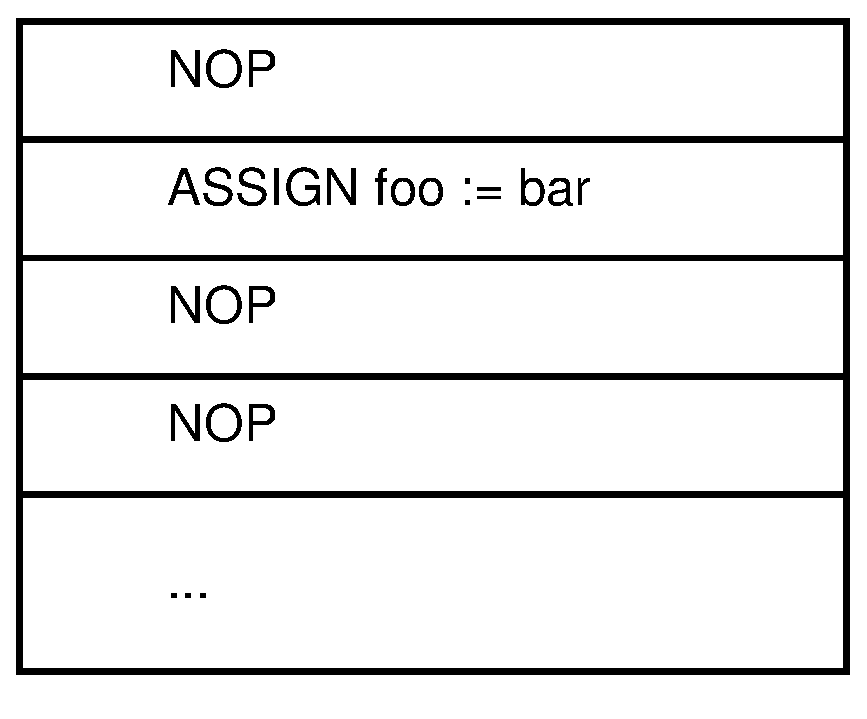
\includegraphics[scale=0.5]{figs/op-log.eps}
\caption{\label{fig:op-log}Operation Log}
\end{figure}

Deciding on a serialisation for operations is done by the operation log. This associates an
``Operation ID'' (OID) with a particular operation. In order to decide on an OID for an operation,
the code picks the next highest instance ID it hasn't seen before and starts a new round of Paxos
for that instance, trying to assert that \verb$OID := <op>$. OIDs are integers and refer to
indexes into an ordered table - the operation log.

I tried a number of different techniques for retrying in the event that the OID was associated
with another operation. Initially I put the retry logic in the database, however it became clear
that it made more sense to create the specification such that once a statement was submitted to
Paxos, it would be entered into the operation log, but at submit time the code could make no
guarantee about the OID the statement would have. This made for a cleaner abstraction interface
between the database and Paxos. The database code now only needed to pass the Paxos layer a
statement/op, and it would receive a callback when that statement was finally entered into the
transaction log, along with the OID it was entered as (which would be the instance ID, as there is
a one-to-one correspondence of OIDs -- instance IDs).

\subsection{Reads}

For a distributed database there is the concept of \emph{fast reads} and \emph{slow reads}. A fast
read is a read that only examines the state of the database locally, without sending anything over
the network.  A slow read involves inserting an operation into the operation log in order to
ensure that the local copy of the database is up to date, then reading from that state.

A fast read has very low latency, as it does not need to send messages to any other nodes, but it
may return out of date data. A slow read forces us to actually examine the current state of the
database by inserting an operation, to ensure we have obtained all transactions issued
prior to the slow read.

In fact, I chose to use a \op{NOP} operation rather than a \op{READ} operation, although they
would semantically be the same (as other nodes do nothing on a \op{READ}), as I felt a \op{NOP}
better represented the operation being sent (do nothing).

\begin{figure}[htb]
\centering
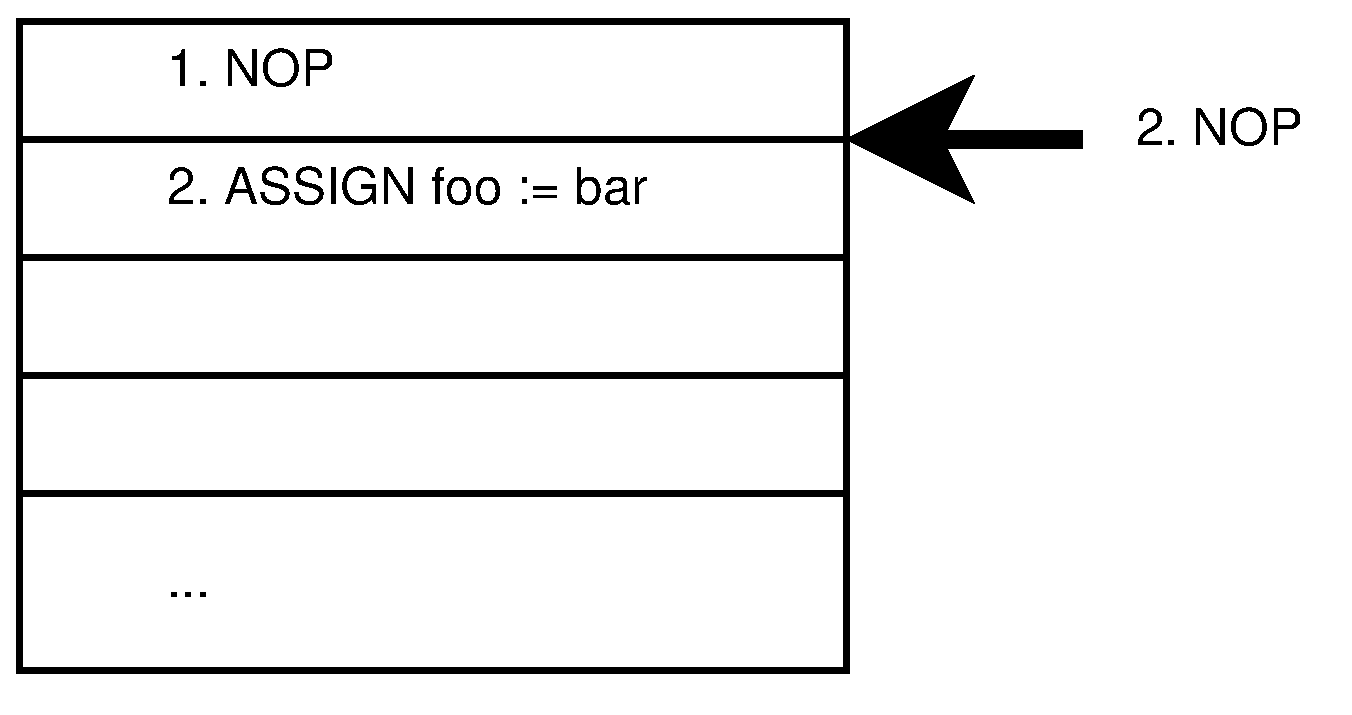
\includegraphics[scale=0.5]{figs/op-log-slow-read-1.eps}
\caption{\label{fig:op-log-slow-read-1}Performing a slow read}
\end{figure}

We can see this from figure~\ref{fig:op-log-slow-read-1}. This is the situation as seen by a node
$N$ at time $t_1$. At time $t_1$ $N$ has only received OID 1 - the \op{ASSIGN} in OID 2 has been
learnt by the network but not by $N$. In order to make sure $N$ is up to date with the network, it
tries to insert a \op{NOP} at OID 2.

As the network has already reached consensus on OID 2, when $N$ tries to set it to a \op{NOP}, the
it will learn the value already obtained by consensus in the network and try and set OID 3 to
\op{NOP} instead. As OID 3 has not had any value set, $N$ succeeds in setting OID 3 to \op{NOP}.

\begin{figure}[htb]
\centering
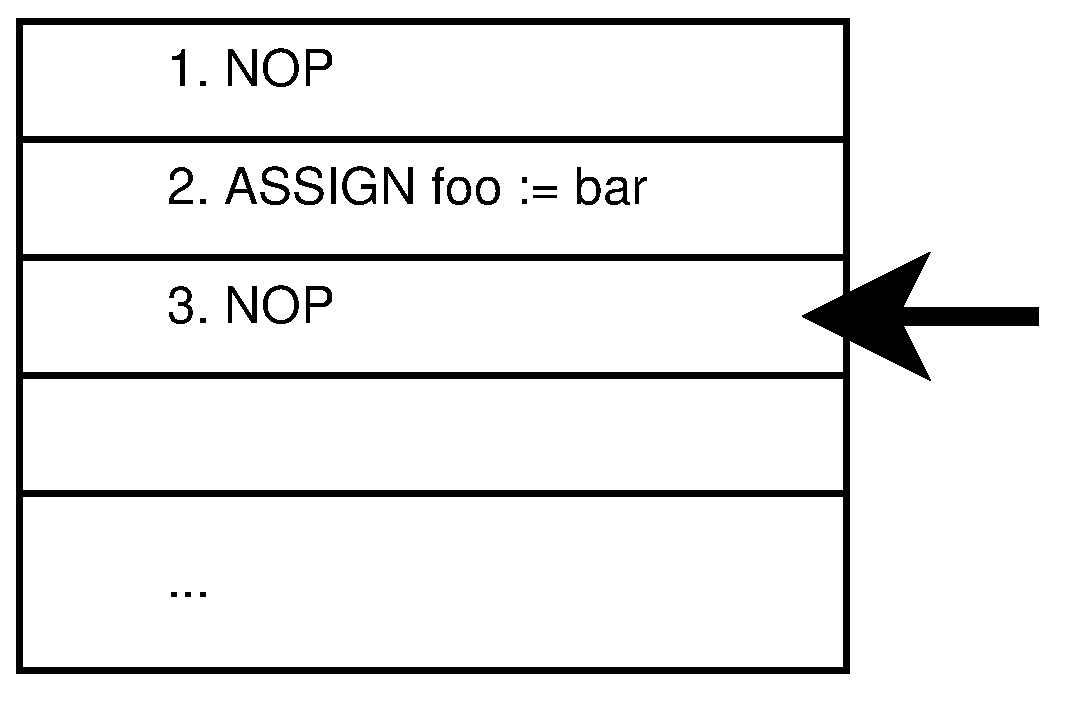
\includegraphics[scale=0.5]{figs/op-log-slow-read-2.eps}
\caption{\label{fig:op-log-slow-read-2}After a slow read}
\end{figure}

In figure~\ref{fig:op-log-slow-read-2} we see the situation at time $t_2$ - the \op{NOP} has been
inserted at OID 3 - from this $N$ can tell that at $t_2$ the latest operation in the op-log is OID
3 - the slow read it just performed.

\subsection{Transactions}

\subsubsection{Global Lock}

\begin{figure}[htb]
\centering
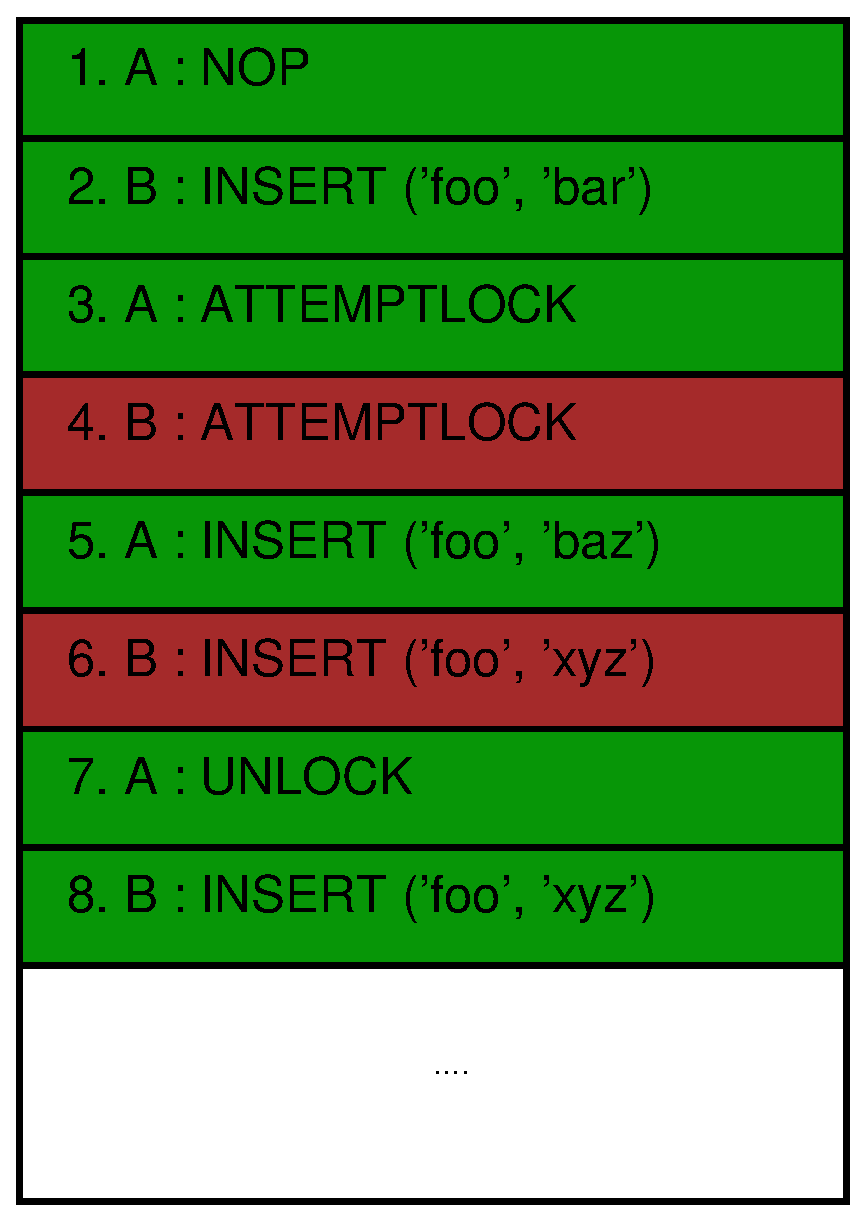
\includegraphics[scale=0.5]{figs/op-log-trylock.eps}
\caption{\label{fig:op-log-trylock}Transactions in the Operation Log}
\end{figure}

% XXX: add brackets to diagram indicating lock holding

My first implementation of transactions was a very na\"ive global lock. In order to start a
transaction, a node inserts the \op{ATTEMPTLOCK} operation. If, when the operation is inserted, the
number of \op{ATTEMPTLOCK}s is well-bracketed (ie, there is an equal number of lock takes and
releases), then the node was successful in taking the lock. While a node holds the lock, no other
node can perform an operation (the operations are inserted in the transaction log but ignored).

As an example, in figure~\ref{fig:op-log-trylock} we can see an operation log with two nodes
performing operations, nodes $A$ and $B$. In OIDs 1 and 2 neither node owns the global lock, so both
nodes are able to freely perform operations. Both try to take the lock and $A$ gets it operation
inserted first as OID 3, so now owns the lock. $B$'s operation is inserted as OID 4, so it has the
semantic meaning of a \op{NOP}. $A$ now performs an assignment under the lock (in reality this
would be a series of operations) as OID 5. As $A$ is the lock holder, the operation is performed.
$B$ tries to perform a different assignment, but as it does not hold the lock, the operation is
not performed. $A$ now releases the lock with an \op{UNLOCK} operation (OID 7). Finally, $B$
retries its assignment, which can finally be performed as no-one now holds the lock.

\subsubsection{Two Phase Locking}

I improved

used two phase locking
take locks in schema order to avoid deadlock and livelock
restart transaction if locks taken out of order

use strict 2PL to avoid cascading aborts

potential further locking schemes?

\section{Database Implementation}

\subsection{SQL}

% XXX: didn't finish - explain!!!

\subsubsection{Grammar}

I implemented SQL parsing using PyParsing, a python library that makes it easy to programmatically
construct simple grammars. Using this I constructed a grammar of the form:

\verb+SELECT (field1,field2,...) WHERE <where-clause>+ \\
\verb+INSERT (value1,value2,...)+ \\
\verb+DELETE WHERE <where-clause>+ \\
\verb+UPDATE SET k1=v1, k2=v2, ... WHERE <where-clause>+ \\

The grammar for the WHERE clause (marked as \verb+<where-clause>+ above) is more complicated and
is presented below in production rules:
\begin{enumerate}
\item \verb+B -> AND | OR+
\item \verb+T -> f op f | ( C )+
\item \verb+C -> T B T | T+
\item \verb+S -> C EOL+
\end{enumerate}

In the above production rules \verb+f+ is either a fieldname, string or integer and \verb+EOL+
refers to the end of the string.

\subsubsection{Recursive Descent Parser}

\begin{figure}[htb]
\centering
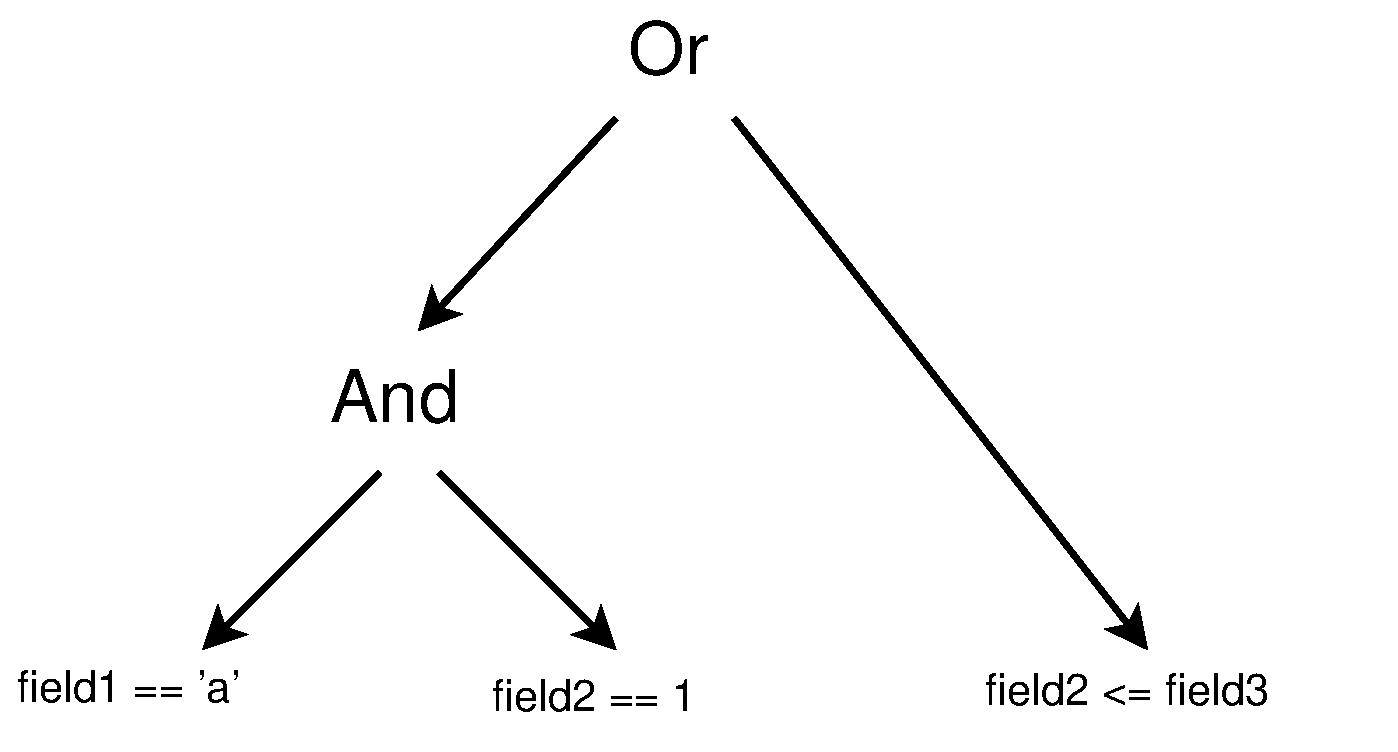
\includegraphics[scale=0.5]{figs/where-ast.eps}
\caption{\label{fig:where-ast}Example WHERE clause matching tree}
\end{figure}

For this grammar I then built a simple recursive descent parser to construct a boolean matching
tree. For example, the SQL fragment \verb+WHERE (field1 == 'a' AND field2 == 1) OR field2 <= field3+
would be parsed into the tree represented by figure~\ref{fig:where-ast}.

% How tools affected things
% Optimisation - ``what it is''
% Talk about iterations
%
% SQL parser
% - what it supports
%
% -start up costs
%   - ping time etc
%   - inefficiencies
%   - cf. ``supernodes'' vs DHTs to organise nodes
%
% Talk about laptop breaking

\section{Testing}

I started off implementing unit tests for the

\subsection{Commandline Tools}

I implemented several commandline tools to interface with the main body of code. As I implemented
Paxos

\cleardoublepage
\chapter{Evaluation}

After designing and implementing the system, I evaluated its performance against a number of
metrics. These were designed to measure how the system's performance differed with regard to
different parameters. The main parameters I varied were the number of nodes in the network and the
number of writers in the network. I also measured how the system performed in a situation with
limited bandwidth, and how the various improvements to the implementation that I made performed
against each other.

\section{Method}

There were a number of metrics I used to evaluate the system. The two main metrics were the
latency of an operation -- how long it took to complete after being issued, and the throughput of
the system -- how many operations could be completed in unit time. I also measured how the
bandwidth used varied in different situations.

\subsection{Simulation}

In order to evaluate the database I decided to simulate the network on a single machine. Initially
I created a separate program for each node, but for all but the most simple network scenarios it
became necessary to run all nodes in the same Python script to programmatically generate results.
I discuss the limitations of this in the section below. There were a number of reasons why it was
necessary to simulate the network on a single machine.

Firstly, it is impractical to create an actual network on a number of computers. Co-ordinating
tests between a large number of machines is difficult, and even being able to use that amount of
resources would be impractical.

Also, as the number of nodes increases, it becomes increasingly difficult to get meaningful
results from nodes run on a physical network, due to other factors such as networking delay. It
also makes results inconsistent and difficult to reproduce on several runs.

\subsubsection*{Assumptions}

For my simulation to be a valid measure of how the network responds, I made certain assumptions.
As a distributed application, I would expect my application to be mainly IO bound, rather than
being CPU bound. IO bound means that the application spends most of the time waiting for IO, in
this case network IO -- sending and receiving messages, as opposed to CPU bound, which means the
application spends most of its time running on the CPU. It is necessary for the application to be
IO bound in order for the simulation to be valid - if it is in fact CPU bound, running multiple
nodes on the same machine will lead to increased CPU load which will mean that the simulation
becomes invalid, as the performance of the simulated nodes deviates from the performance of a real
network.

However, as I am simulating a network on one computer, this assumption does begin to
break down as the number of nodes increases. This problem is exacerbated because Python is
limited to only using one core without explicit parallelism, and Twisted's event loop runs
for not just one node but for all the nodes in the network. A potential fix to would be to spawn
different threads for each node and then join the results when the simulation is done. In this way
the simulation could utilise the full resources of the simulating machine, instead of being
artificially. While this is possible in Twisted, it is not straightforward, and unfortunately time
constraints did not allow further exploration of this evaluation method.

\subsection{Ratelimiting}

talk about ratelimiting
networking delay

Unfortunately, my application had no congestion control or flow control built into the protocol.
While this would be a potential advantage of TCP, other features of TCP would be unnecessary, as
Paxos is decided to deal with message loss, and TCP provides reliable message delivery. So a
potential improvement would be to build Paxos on top of another protocol built on UDP, which
provides congestion control and flow control on the layer underneath, but without providing
unnecessary features such as reliable message delivery.


\subsection{Gathering and Formatting Results}

To generate the results, I ran a simulation of the network and generated the data points
necessary. I then performed some simple statistical methods on it, and output it to a datafile. I
then used gnuplot to format the data into a graph which I could then embed in my dissertation. I
used this method so that it was very straightforward to regenerate the graph automatically,
without having to perform manual tweaking, which would be very time consuming.

I wrote a script that performed the actual simulation and output the data. It took a number of
commandline parameters, specifying the number of nodes in the network, the number of writers, the
number of operations to perform and the type of operations. It then constructed this network and
bootstrapped it. It could not immediately run the operations, but had to wait for every node in
the network to be aware of other nodes in the network. This start up time was not reflected in the
results. After the network bootstrapped, the script started the required number of nodes writing,
and recorded the relevant metric in a CSV file.

I ran this script 5 times for each statistic, and then calculated the average and standard
deviation for each point using another script. The output of this was then put in a datafile
suitable for gnuplot to process.

Finally I ran a gnuplot script which generated a graph for the datafile. It handled formatting and
plotting the graph. This was all co-ordinated from a Makefile, so that with a single command I
could regenerate all graphs necessary. This automation meant I could review my data generation
process thoroughly to be sure it was valid, and be sure that I was handling all the data
consistently.

\section{Contention}

I started off by measuring how the network responds to contention in the network. This means that
measuring how the latency and throughput of the network change in response to the number of nodes
in the network which are writing.

\subsection{Latency}

\paragraph{5 Nodes}

\begin{figure}[htb]
\centering
\lwincludegraphics[scale=2]{figs/lat_5.eps}
\caption{\label{fig:lat-5}Latency for 5 Nodes}
\end{figure}

Firstly I measured a network with 5 nodes. Figure~\ref{fig:lat-5} shows the number of writers vs
the average latency of an operation. There are three lines plotted on the graph, corresponding to
three different types of network operations. Firstly the latency of a pure Paxos is plotted. On
top of this is plotted the latency of a single database operation. This is very close to the Paxos
latency. This is expected as a database operation is simply a specific Paxos operation, so the
minor difference is due to the database processing overhead. As mentioned in the Method section,
we expect this overhead to minor, as the application is mainly IO bound rather than CPU bound.
However, a small amount of added CPU latency is not unexpected. However, the third line plots a
database transaction, which has significantly more latency. This is because a transaction involves
waiting on several Paxos operations to be committed before it is considered done.

However, in all cases we can see that the latency of committing an operation to the
network increases linearly with the number of writers in the network, with a very strong
correlation.

\paragraph{20 Nodes}

\begin{figure}[htb]
\centering
\lwincludegraphics[scale=2]{figs/lat_20.eps}
\caption{\label{fig:lat-20}Latency for 20 Nodes}
\end{figure}

I repeated this experiment with a network of 20 nodes


In figure~\ref{fig:lat-20} we can see that the throughput of the network decreases
exponentially with the number of concurrent writers in the system. We can also see that while
there is little overhead from using the database layer over the top of Paxos, there is substantial
overhead performing multiple transactions.

\paragraph{Network Size}

\begin{figure}[htb]
\centering
\lwincludegraphics[scale=2]{figs/lat_rev.eps}
\caption{\label{fig:latency-rev}Latency vs Network Size}
\end{figure}

I also measured how the network response time is affected by the number of nodes in the network.
Using only a single writer, I measured the latency for networks of varying sizes. This is
displayed in figure~\ref{fig:latency-rev}.

\subsection{Throughput}

Next I measured the throughput of the network. This is the number of operations per second that
can be processed by the network. Again I plotted three lines for each graph -- paxos throughput,
database operation throughput and database transaction throughput.

I measured the throughput by measuring how long it took to commit 5 operations to the network with
a given number of writers. I did this 5 times for each writer and then took the average and
standard deviation of each point. I then plotted $5/x$ for each point as the average throughput in
\emph{operation seconds\superscript{-1}}.

\paragraph{5 Nodes}

\begin{figure}[htb]
\centering
\lwincludegraphics[scale=2]{figs/thru_5.eps}
\caption{\label{fig:thruput-5}Throughput for 5 Nodes}
\end{figure}

Again I initially did this for a network of 5 nodes. The results of this are in
figure~\ref{fig:thruput-5}. We can see that the throughput of the network decreases with
$\frac{1}{w}$, where $w$ is the number of concurrent writers in the system. Again the performance of
Paxos and database operations is similar, with very similar throughputs. However there is still a
big overhead to using transactions, as evidenced from the substantially reduced throughput,
reduced by nearly a factor of 5.

\paragraph{20 Nodes}

\begin{figure}[htb]
\centering
\lwincludegraphics[scale=2]{figs/thru_20.eps}
\caption{\label{fig:thruput-20}Throughput for 20 Nodes}
\end{figure}

In figure~\ref{fig:thruput-20} we can see that the throughput of the network decreases
exponentially with the number of concurrent writers in the system. We can also see that while
there is little overhead from using the database layer over the top of Paxos, there is substantial
overhead performing multiple transactions.

\begin{figure}[htb]
\centering
\lwincludegraphics[scale=2]{figs/thru_rev.eps}
\caption{\label{fig:thruput-rev}Throughput vs Network size}
\end{figure}

\subsection{Start up costs}

As the size of the network increases the cost of bootstrapping the network becomes prohibitively
expensive

\begin{figure}[htb]
\centering
\lwincludegraphics[scale=2]{figs/start.eps}
\caption{\label{fig:start}Start}
\end{figure}


\begin{figure}[htb]
\centering
\lwincludegraphics[scale=2]{figs/start2.eps}
\caption{\label{fig:start2}Start 2}
\end{figure}


\subsubsection{$N^2$}

\subsubsection{Sublinear}



\section{Limitations}

% XXX: rewrite
The main limitation of the system is its speed. In particular, transactions, a core component of
any database, have a large cost.

Another limitation is the lack of stable storage support in the database. Although it supports
durability in that, if a node leaves, and then returns, the operation will persist in the network
and if that node rejoins, then it will see the transaction again, if a majority of nodes leave and
rejoin, the database will lose its transactions as it has no stable storage and a majority of
nodes have failed. However if the nodes leave slowly enough for the network quorum to adjust it
will be fine.

Another drawback is that the network struggles to function as its size increases - the way I have
implemented Paxos is easy to debug but is very ``chatty''. Using a more efficient variant such as
MultiPaxos would decrease the bandwidth requirements of the system. Alternatively using a variant
such as FastPaxos would decrease the latency.

Although I show an improvement to the startup cost of bootstrapping the network, my improvement
only centralises the bootstrapping, losing all the advantages of using a distributed network. A
complete solution would be to use a DHT or super-node hierarchy.

Due to time constraints I did not have time to implement all the SQL syntax that my requirements
indicated. However this is not a significant concern as it is relatively easy to add new syntax and
operations to the database.

\section{Changes with hindsight}

If I was to do the project again, there are several large changes that I would make. These mainly
are design choices more than anything else. One big design choice I made was to use an
asynchronous programming paradigm. I chose this because I thought it would make the project
simpler and quicker to write, by leveraging Twisted's network stack. However I didn't allow for
the difficulty of understanding and designing Paxos, or a database, or Paxos and a database under
a new programming paradigm.

Another design problem was that I started with a key/value database prototype, and later
refactored it into a row based database. I then added an SQL interface and layered transactions on
top. This was a reasonable choice, as I started small and then worked bigger, but in retrospect
the system should have been row-based from the start. The SQL interface should have been more
tightly integrated rather than less tightly, and transactions should have been the core aspect of
my system, rather than a layering of operations. However it is difficult to predict how the
project would have turned out with this plan, it is not necessarily as easy to implement as it
sounds and I believe my choices were very reasonable at the time.

Another possibility is that I should have started with smaller prototypes of the complete system,
rather than prototypes of both of them that were then joined. A disadvantage of my approach was
that as my understanding of how the design would work progressed, the API interface between the
two components changed significantly and repeated. This led to problems with testing, and with
having to rewrite various user interfaces repeatedly. An alternative approach could have been to
use an agile programming strategy, rather than an iterative one. A quote that summarises my
experience with my project is by Fred Brooks: ``plan to throw one away; you will, anyhow''.

\subsection*{Twisted}

In retrospect, if I was to do the project again I would probably not use Twisted. Twisted provided
me with a powerful framework for building an asynchronous network application, but it had
disadvantages as well as advantages, which I will briefly outline.

I had to learn a lot for this project. I had to learn and understand how how Paxos works and
design a protocol that implements it. I also had to learn and understand the basics of building a
database, and on top of that - a distributed database. Twisted has a high learning curve, and I
ended up investing a lot of time understanding how to work with Twisted and in some cases working
against it. I spent lots of time interfacing with it, some of which was unnecessary.

It is difficult to know how much networking code Twisted saved me writing, however
the message requirements of paxos are quite simple, and I think that with a few days work making
some helper network classes much of the complexity of using and interfacing with Twisted could
have been avoided. Certainly there are cases when debugging would have been easier, and I feel my
project would have been less ``heavy-weight'', particularly when it came to unit tests, another
problem I will discuss later.

As I worked through several prototype versions, Twisted became cumbersome to use. I had to keep
learning new parts of it, which was frustrating to have to keep delving into the innards of it,
particularly as I started to feel that it hadn't helped me as much as I had anticipated.

Using the asynchronous paradigm initially helped me reason about Paxos and how I would design my
system, however later on I felt the asynchronous model was unnecessary, and Twisted became
superfluous. Certainly my project would have been very different without the decision to use it.

\subsection*{Testing}

Unit tests became a problem as I progressed through the project.  They became a hindrance, as I
was refactoring my code base often, they were not that effective. Test Driven Development may have
been a better choice, as I wrote my unit tests after I had written the code, I would often write
the code, write the tests, it would all work. Then I would refactor the code, rewrite the tests --
every refactoring would invalidate large numbers of tests. This was also due to how tightly
coupled my code was with Twisted. This is another reason I would reconsider my decision to use
Twisted if I were to redo the project.

\section{Summary}

In summary, my project had clear successes but also some clear drawbacks. I effectively
implemented Paxos, and built an ACID distributed database on top, with support for transactions. I
made some improvements to my design, but ultimately there are still many more clear avenues for
improvement. The project suffers from inefficiency, and is slow, but is an effective prototype
that gives valuable insight into the performance ramifications of different design decisions of a
distributed database. My project was limited not just by the limited amount of time I had, but
also by my lack of expertise in the area, and I have gained valuable insights into my decisions
and how I would improve the project if I were to implement it again.


\cleardoublepage
\chapter{Conclusion}

In summary, I successfully completed both an implementation of the Paxos protocol and a
distributed database on top. The theory behind the design and the requirements are set out in the
Preparation Chapter. The design and implementation of these two components is discussed in detail
in the Implementation Chapter. Both were designed simply, and this led to various inefficiencies
and tradeoffs that I measured and quantitatively evaluated in the Evaluation Chapter, also
discussing the limitations of the project. Here I will outline the formal success criteria and how
my project compares with them, as well as proposing potential extensions or improvements that
could be investigated further.

\section{Comparison with Requirements}

The requirements described in Chapter 2 are a formal list of elements of the project to be
considered in evaluating its success. I will outline them here and discuss how each was realised,
and to what extent.

\subsection{Paxos}

The project successfully meets the requirements of being able to form a running network which can
achieve consensus. It can perform dynamic leader election through the Paxos network, and
supports nodes joining and leaving arbitrarily. This area of the success criteria was met fully.

\subsection{ACID}

The ACID success criterion was to support all ACID properties - Atomic, Consistent, Isolated and
Durable. The project supports all of them as long as the network persists - there is no support
for stable storage.

\subsection{SQL}

The success criterion for SQL was designed to reduce the scope of SQL in order to allow me to
focus on the design of the Paxos protocol and the database. It was reduced to a single table with
a static name, SELECT and INSERT statements, including a WHERE clause, and GROUP BY, ORDER BY and
aggregation. The latter three of these I did not implement, due to time constraints. I decided to
focus on Paxos and the database rather than on implementing SQL, as I felt they were the core of
my project and SQL merely an interface for it. However I did successfully implement the first
three elements of this criterion, that is, the SELECT and INSERT statements with a table name, and
a recursive descent WHERE clause parser.

\section{Further Work}

There are multiple opportunities that could be investigated given more time that would allow for
the project to be improved and extended.

\subsection{Transactions}

Transactions are a core component of databases today, and one of the foundations of ACID - a key
requirement of mine. As it stands, transactions are the weakest part of my project. There are
several different locking schemes that could be used instead of the basic ones used in my project,
Optimistic Concurrency Control (OCC) being one of particular interest, as it is much more
effective in a network with low contention.

\subsection{Durability}

A large part of contemporary database design involves ensuring that database operations persist
ie, durability - the ``D'' from ACID. My project did not support stable storage as a means of
ensuring durability and extending this, through the use of write-ahead logs (WAL) and or shadow
paging, would be a high priority given more time.

\subsection{Network Hierarchy}

A clear problem during evaluation was the effect of the network size on the amount of time and the
amount of bandwidth used to bootstrap the network. Increasing the size beyond a certain number of
nodes led to large slow downs in the network, that in the real world would have serious practical
implications on the efficacy of the network.

For large peer-to-peer networks there are several mature techniques that could be used to manage a
network of scale efficiently. One of these is using ``supernodes'' -- nodes designated either
through bandwidth or chosen randomly to co-ordinate their child nodes, reducing the message
overhead from $N^2$ to $S^2$ where $S$ is the number of supernodes. Another technique is the use
of Distributed Hashing Tables (DHTs) to manage nodes. This involves computing a measure or
pseudo-measure of ``distance'' to other nodes, then having nodes only contact their
``neighbours'', rather than the entire network.

Either of these would be much more efficient to manage the network than the current $N^2$ na\"ive
approach.

\subsection{SQL}

Although I had planned to support a more comprehensive subset of SQL syntax, time constraints meant
that I was unable to do so. A more complete database solution would include aggregation support,
as well as \verb+ORDER BY+ and \verb+GROUP BY+ clauses.

\subsection{MultiPaxos}

My implementation of MultiPaxos was limited by the amount of time I had to implement the project,
and the difficulty I had initially understanding the Paxos and MultiPaxos protocol. Redesigning
the project to support the more efficient MultiPaxos and FastPaxos variants would allow an
increase in efficiency both in terms of network throughput and latency, and also in terms of
bandwidth.

\subsection{Security}

One area of Computer Science that I constantly encountered during this project was security.
Although I decided it was beyond the scope of my project, given more time it would have been
valuable to investigate the security implications of many of my design decisions and build more
security into my design, as well as considering implementing Byzantine Paxos, which can tolerate
rogue and faulty nodes in the network.

\cleardoublepage

%%%%%%%%%%%%%%%%%%%%%%%%%%%%%%%%%%%%%%%%%%%%%%%%%%%%%%%%%%%%%%%%%%%%%
% the bibliography

\addcontentsline{toc}{chapter}{Bibliography}
\bibliography{refs}
\cleardoublepage

%%%%%%%%%%%%%%%%%%%%%%%%%%%%%%%%%%%%%%%%%%%%%%%%%%%%%%%%%%%%%%%%%%%%%
% the appendices
\appendix

\chapter{Project Proposal}

\vfil

\centerline{\Large Computer Science Project Proposal}
\vspace{0.4in}
\centerline{\Large PDB: A Distributed Database Based on Paxos}
\vspace{0.4in}
\centerline{\large Charlie Shepherd, Churchill College}
\vspace{0.3in}
\centerline{\large Originator: Charlie Shepherd}
\vspace{0.3in}
\centerline{\large 18$^{th}$ October 2012}

\vfil


\noindent
{\bf Project Supervisor:} Stephen Cross
\vspace{0.2in}

\noindent
{\bf Director of Studies:} Dr John Fawcett
\vspace{0.2in}
\noindent

\noindent
{\bf Project Overseers:} Dr~A.~Madhavapeddy \& Dr~M.~Kuhn


% Main document

\section*{Introduction, The Problem To Be Addressed}

{\em Paxos} is a protocol for achieving distributed consensus, developed by Leslie Lamport in 1991.

The motivation for Paxos as a protocol is that it is capable of handling failures that other
consensus protocols cannot. {\em Two Phase Commit} (2PC) and {\em Three Phase Commit} (3PC) are two common
protocols that can be used to ensure atomic commits in a distributed system.

2PC works by having a co-ordinator node contact every node and send a proposal message. Each node
must then either respond with a commit or abort message. However, 2PC suffers from several
problems, mainly that it is a blocking protocol. This means that if the co-ordinator fails, and
then a node subsequently fails, the network will deadlock, as 2PC is not able to recover from that
failure situation.

3PC is an extension to 2PC which endeavours to fix this limitation, at the expense of greater
latency, by adding a third roundtrip to confirm the commit to all nodes. This means that the
protocol is asynchronous, and that node failures cannot block the protocol or cause it to fail.
However, it still has its own limitations, in particular, in the event of a network partition. If
the network is partitioned so that in one partition all nodes vote ``commit'' and in the other all
nodes vote ``abort'' both partitions will initiate recovery, and when the network merges again the
system will be in an inconsistent state. This is the limitation that Paxos was intended to solve.

My project will be to design and implement a distributed database, built on the Paxos protocol.


\section*{Starting Point}

My starting point will be to study the Paxos protocol, as well as research distributed databases.
From there I will develop a library implementing Paxos, along with unit tests. I will then design
and implement a distributed database on the Paxos library. The challenge will be to implement a
complex distributed protocol and then utilise it for a database, as these are both areas I have
little experience of.

\section*{Resources Required}

I will mainly do my project on a virtual machine which is running on my own personal laptop.
The source code will be committed to a Git repository, which will be pushed to Bitbucket and my
own personal host. The virtual machine contents will be backed up on an external HDD for quick
recovery, although the git repository will be adequate for restoring my project if the system I am
developing it on fails.
I require no other special resources.

\section*{Work to be done}

The project breaks down into the following sub-projects:

\begin{enumerate}

\item A study of distributed algorithms and the Paxos protocol

\item A study of distributed databases

\item Implementing the Paxos protocol

\item Designing the distributed database

\item Implementing the distributed database

\item Evaluating the performance of the database

\end{enumerate}

\section*{Success Criteria for the Main Result}

In order for the project to be a success, the following must be true:

\begin{enumerate}

\item The project must correctly implement the Paxos protocol.
	The library must be capable of forming a running network,
	in particular dynamic leader election,
	as well as achieving consensus on a key/value store across the network.

\item The database must implement a subset of SQL, specifically:
\begin{enumerate}
\item A single table with a static name
\item SELECT/INSERT
\item WHERE
\item GROUP BY
\item ORDER BY
\item Aggregation
\end{enumerate}

\item The database must have all ACID properties, that is:
\begin{enumerate}
\item Atomic
\item Consistent
\item Isolated
\item Durable
\end{enumerate}

\end{enumerate}

\section*{Evaluation Topics}

There are several potential evaluation metrics for the project.

One major metric is transaction latency - the time for a transaction to be committed to the system. This
can be evaluated in a number of difference circumstances, including simulated node failure, leader
failure and network partition, and the results analysed to see how the system handles performance
under failure compared to normal conditions.

Another key metric is transaction throughput - the maximum number of transactions committed to the
network over a specified period of time. Again there are a number of different situations
throughput can be measured in, including load from one source, load from multiple sources and
load under failure.

I will also investigate the advantages of a distributed database over a normal single-server
database, particularly in terms of scalability. I will also consider how performance is affected
by the ratio of writing clients to reading clients.

\section*{Possible Extensions}

A clear possible extension is to investigate various different modifications to Paxos in order
to try to optimise the database for certain performance characteristics
(e.g. fast reads, but slow writes),
and to assess the usefulness and efficiency of these modifications.

Another possible extension is to investigate how the database performs when various ACID
properties are relaxed, and to measure and analyse how the performance gains compare with the
tradeoffs made.


\section*{Timetable: Workplan and Milestones to be achieved.}

\setlength\parindent{0pt}
\parskip = \baselineskip

Planned starting date is 19/10/2011.

\subsection*{Michaelmas Term}

{\bf 19/10/2012-01/11/2012} Research distributed algorithms and the Paxos protocol; design the
protocol implementation and library layout.

Milestone: A write up of the Paxos algorithm and a design document of the implementation.

{\bf 02/11/2012-15/11/2012} Begin the protocol implementation.

Milestone: Basic Paxos implementation.

{\bf 16/11/2012-29/11/2012} Finish implementation of Paxos library.

Milestone: Paxos implementation that can coordinate distributed leader election and achieve
consensus, including unit tests.

\subsection*{Christmas Vacation}

{\bf 30/11/2012-13/12/2012} Research distributed databases and design the database implementation.

Milestone: A write up of research on distributed databases and a design document for the database.

{\bf 14/12/2012-27/12/2012} Slack time/Revision/Holiday break.

{\bf 28/12/2012-10/01/2013} Prepare for progress report, start database implementation.

Milestone: Draft progress report, initial database implementation.

\subsection*{Lent Term}
{\bf 11/01/2013-24/01/2013} Write progress report, finish database implementation.

Milestone: Finished Progress report, fully functional database implementation.
Deadlines: Progress report deadline - 01/02/2013.

{\bf 25/01/2013-07/02/2013} Perform initial performance analysis on transaction, including
transaction latency and transaction throughput.

Milestone: Initial analysis data.

{\bf 08/02/2013-21/02/2013} Perform detailed performance analysis comparing distributed and
centralised servers, and on failing and partitioned networks.

Milestone: Analysis data on server models and on performance during failure.

{\bf 22/02/2013-07/03/2013} Investigate improvements to the protocol/implementation and their effect on
performance metrics.

Milestone: Improvements to protocol/implementation and revised performance data.

{\bf 08/03/2013-21/03/2013} Start dissertation.

Milestone: Draft Introduction and Preparation sections complete.

\subsection*{Easter Vacation}

{\bf 22/03/2013-04/04/2013} Finish writing up dissertation.

Milestone: Draft Implementation, Evaluation and Conclusion sections complete.

{\bf 05/04/2013-18/04/2013} Proof reading and then an early submission so as to concentrate on
examination revision.

Milestone: Finished dissertation.

\subsection*{Easter Term}
{\bf 19/04/2013-02/05/2013} Slack time/Revision/Holiday break.

{\bf 03/05/2013-16/05/2013} Slack time/Revision/Holiday break.

Deadlines: Official dissertation submission deadline - 17/05/2013.


\end{document}
